%! TeX program = pdflatex

%%%%%%%%%%%%%%%%%%%%%%%%%%%%%%%%%%%%%%%%%
% Wenneker Assignment
% LaTeX Template
% Version 2.0 (12/1/2019)
%
% This template originates from:
% http://www.LaTeXTemplates.com
%
% Authors:
% Vel (vel@LaTeXTemplates.com)
% Frits Wenneker
%
% License:
% CC BY-NC-SA 3.0 (http://creativecommons.org/licenses/by-nc-sa/3.0/)
% 
%%%%%%%%%%%%%%%%%%%%%%%%%%%%%%%%%%%%%%%%%

%----------------------------------------------------------------------------------------
%	PACKAGES AND OTHER DOCUMENT CONFIGURATIONS
%----------------------------------------------------------------------------------------


\documentclass[11pt]{scrartcl} % Font size

%%%%%%%%%%%%%%%%%%%%%%%%%%%%%%%%%%%%%%%%%
% Wenneker Assignment
% Structure Specification File
% Version 2.0 (12/1/2019)
%
% This template originates from:
% http://www.LaTeXTemplates.com
%
% Authors:
% Vel (vel@LaTeXTemplates.com)
% Frits Wenneker
%
% License:
% CC BY-NC-SA 3.0 (http://creativecommons.org/licenses/by-nc-sa/3.0/)
% 
%%%%%%%%%%%%%%%%%%%%%%%%%%%%%%%%%%%%%%%%%

%----------------------------------------------------------------------------------------
%	PACKAGES AND OTHER DOCUMENT CONFIGURATIONS
%----------------------------------------------------------------------------------------

\usepackage{amsmath, amsfonts, amsthm} % Math packages

\usepackage{listings} % Code listings, with syntax highlighting

\usepackage[english]{babel} % English language hyphenation

\usepackage{graphicx} % Required for inserting images
\graphicspath{{Figures/}{./}} % Specifies where to look for included images (trailing slash required)

\usepackage{booktabs} % Required for better horizontal rules in tables

\numberwithin{equation}{section} % Number equations within sections (i.e. 1.1, 1.2, 2.1, 2.2 instead of 1, 2, 3, 4)
\numberwithin{figure}{section} % Number figures within sections (i.e. 1.1, 1.2, 2.1, 2.2 instead of 1, 2, 3, 4)
\numberwithin{table}{section} % Number tables within sections (i.e. 1.1, 1.2, 2.1, 2.2 instead of 1, 2, 3, 4)

\setlength\parindent{0pt} % Removes all indentation from paragraphs

\usepackage{enumitem} % Required for list customisation
\setlist{noitemsep} % No spacing between list items

%----------------------------------------------------------------------------------------
%	DOCUMENT MARGINS
%----------------------------------------------------------------------------------------

\usepackage{geometry} % Required for adjusting page dimensions and margins

\geometry{
	paper=a4paper, % Paper size, change to letterpaper for US letter size
	top=2.5cm, % Top margin
	bottom=3cm, % Bottom margin
	left=3cm, % Left margin
	right=3cm, % Right margin
	headheight=0.75cm, % Header height
	footskip=1.5cm, % Space from the bottom margin to the baseline of the footer
	headsep=0.75cm, % Space from the top margin to the baseline of the header
	%showframe, % Uncomment to show how the type block is set on the page
}

%----------------------------------------------------------------------------------------
%	FONTS
%----------------------------------------------------------------------------------------

\usepackage[utf8]{inputenc} % Required for inputting international characters
\usepackage[T1]{fontenc} % Use 8-bit encoding

\usepackage{fourier} % Use the Adobe Utopia font for the document

%----------------------------------------------------------------------------------------
%	SECTION TITLES
%----------------------------------------------------------------------------------------

\usepackage{sectsty} % Allows customising section commands

\sectionfont{\vspace{6pt}\centering\normalfont\scshape} % \section{} styling
\subsectionfont{\normalfont\bfseries} % \subsection{} styling
\subsubsectionfont{\normalfont\itshape} % \subsubsection{} styling
\paragraphfont{\normalfont\scshape} % \paragraph{} styling

%----------------------------------------------------------------------------------------
%	HEADERS AND FOOTERS
%----------------------------------------------------------------------------------------

\usepackage{scrlayer-scrpage} % Required for customising headers and footers

\ohead*{} % Right header
\ihead*{} % Left header
\chead*{} % Centre header

\ofoot*{} % Right footer
\ifoot*{} % Left footer
\cfoot*{\pagemark} % Centre footer

% \usepackage{minted}
\usepackage[outputdir=build]{minted}
\usepackage{xcolor}

\definecolor{colorVHDL}{RGB}{220, 212, 255}
\definecolor{colorPy}{RGB}{237, 255, 176}
\definecolor{negro}{rgb}{0,0,0}
\definecolor{null}{rgb}{1,1,1}
\newmintedfile[inputmintedVHDL]{vhdl}{linenos=true,bgcolor = colorVHDL, breaklines = true, frame = single}
% \newmintedfile[inputmintedPy]{python}{linenos=true, bgcolor = colorPy, breaklines = true,frame = single}
\newmintedfile[inputmintedPy]{python}{linenos=true, bgcolor = negro, breaklines = true,frame = single,rulecolor = null,breakanywhere = true}


\usemintedstyle[python]{monokai}
% ,frame=single,framerule=1pt

% \usepackage{tcolorbox}
% \usepackage{etoolbox}
% \BeforeBeginEnvironment{minted}{\begin{tcolorbox}}%
% \AfterEndEnvironment{minted}{\end{tcolorbox}}%




\usepackage[active,tightpage]{preview}

\renewcommand{\PreviewBorder}{1in}

\newcommand{\Newpage}{\end{preview}\begin{preview}}

\usepackage{lipsum} % Include the file specifying the document structure and custom commands

%----------------------------------------------------------------------------------------
%	TITLE SECTION
%----------------------------------------------------------------------------------------

% \title{	
% 	\normalfont\normalsize
% 	\textsc{Universidad de Sevilla, Máster de Telecomunicación}\\ % Your university, school and/or department name(s)
% 	\vspace{25pt} % Whitespace
% 	\rule{\linewidth}{0.5pt}\\ % Thin top horizontal rule
% 	\vspace{20pt} % Whitespace
% 	{\huge Modelado y simulación de propagación de pulsos por medios dispersivos en régimen lineal}\\ % The assignment title
% 	\vspace{12pt} % Whitespace
% 	\rule{\linewidth}{2pt}\\ % Thick bottom horizontal rule
% 	\vspace{12pt} % Whitespace
% }

% \documentclass[11pt]{report}
\usepackage{outline} \usepackage{pmgraph} \usepackage[normalem]{ulem}
\usepackage{graphicx} \usepackage{verbatim}
\title{

\includegraphics[width=6cm]{Figures/Logo_US.png} \\
\vspace*{1in}
\textbf{Proyecto estimador de canal OFDM en VHDL}}
\author{Miguel Nogales González-Regueral \\
		\vspace*{0.5in} \\
		Escuela Técnica Superior de Ingeniería\\
        \textbf{Universidad de Sevilla}\\
        Sevilla, España
       } \date{\today}

\vspace{50pt}

%--------------------Make usable space all of page
\setlength{\oddsidemargin}{0in} \setlength{\evensidemargin}{0in}
\setlength{\topmargin}{0in}     \setlength{\headsep}{-.25in}
\setlength{\textwidth}{6.5in}   \setlength{\textheight}{8.5in}
%--------------------Indention
\setlength{\parindent}{1cm}

\begin{document}
\begin{preview}

\maketitle % Print the title

\Newpage

\section{Introducción}

Esta memoria servirá para detallar la funcionalidad de los códigos usados para la parte sobre programación en VHDL y verificación de la asignatura "Electrónica Digital para Comunicaciones" de 1º de MUIT y será presentada junto a otra memoria complementaria sobre códigos Matlab. 

Casi la totalidad de los \emph{test benchs} que se presentarán han sido realizados con la herramienta de \emph{software} libre \emph{CoCoTb} (COroutine based COsimulation TestBench) mientras que los pocos restantes se han realizado en VHDL. Se ha elegido CoCoTb para hacer el proyecto debido a su flexibilidad y su potencial a la hora de realizar simulaciones de código, mucho mas profunda que los que se pueden realizar en VHDL, añadiendo a las simulaciones la potencia de las infinitas librerias que ofrece python para realizar casi cualquier tipo de función.

El proyecto de la asignatura trata de realizar un estimador de canal enteramente en VHDL y opcionalmente complementarlo con la equalización, además de realizar verificación del funcionamiento de los códigos aportados. Esta memoria se estructurará de forma que se mostrarán los códigos de los bloques principales, con comentarios para explicar su funcionalidad en el propio fichero, y se darán breves explicaciones en la memoria de las elecciones de diseño mas relevantes. Primero una sección hablando del diseño del sistema. Posteriormente se analizarán los bloques funcionales con pequeños trozos de códigos especialmente llamativos, para acabar con un resumen de hitos y mejoras. Se añade un anexo con los códigos tanto de VHDL como de Python para verificar.

\section{Estimador de canal, diseño de la estructura}

En la asignatura se ha propuesto una posible implementación del sistema, pero en este trabajo se ha optado por diseñar otra desde cero, y dentro de lo posible mejorarla y añadirle ventajas que la hagan útil para determinado caso.

De esta manera, se ha desarrollado un esquema en el cual se elimina, con respecto a la propuesta original, cualquier uso de memorias DRAM y máquinas de estados, haciendo el sistema más simple y, al no necesitar estados, más rápido. Esto ha facilitado bastante la programación en VHDL, pero a coste de dificultad en el diseño, teniendo que salvar varias trabas tomando enfoques diferentes. De esta forma, se ha logrado tener el sistema funcionando bajo una arquitectura en \emph{pipeline}, haciendolo una implementación mucho más eficiente, efectiva y requiriendo menos dispositivos. En la Figura \ref{implementacion} se muestra el diagrama de bloques de está implementación.

% \begin{figure}[!h] % [h] forces the figure to be output where it is defined in the code (it suppresses floating)
% 	\centering
% 	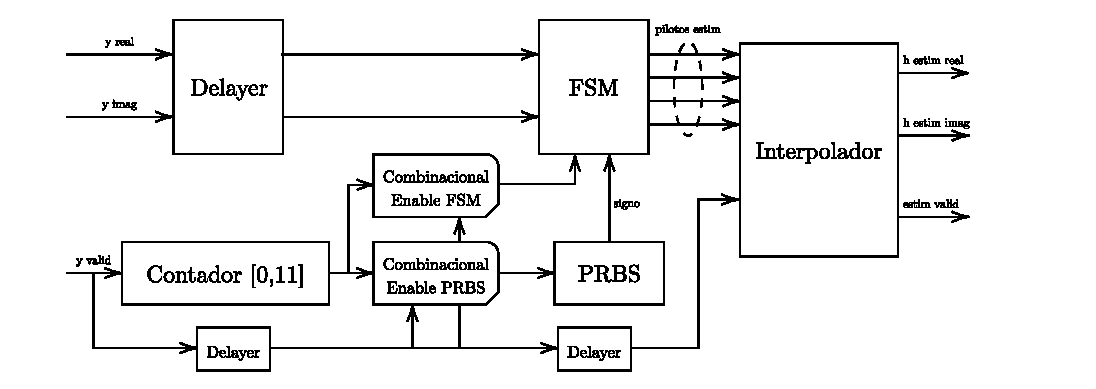
\includegraphics[width=1\columnwidth,trim={0 0 1cm 0},clip]{./Figures/Diagrama1.pdf} % Example image
% 	\caption{Esquema del estimador del canal.}
% 	\label{implementacion}
% \end{figure}

\begin{minipage}{\linewidth}
	\begin{center}
		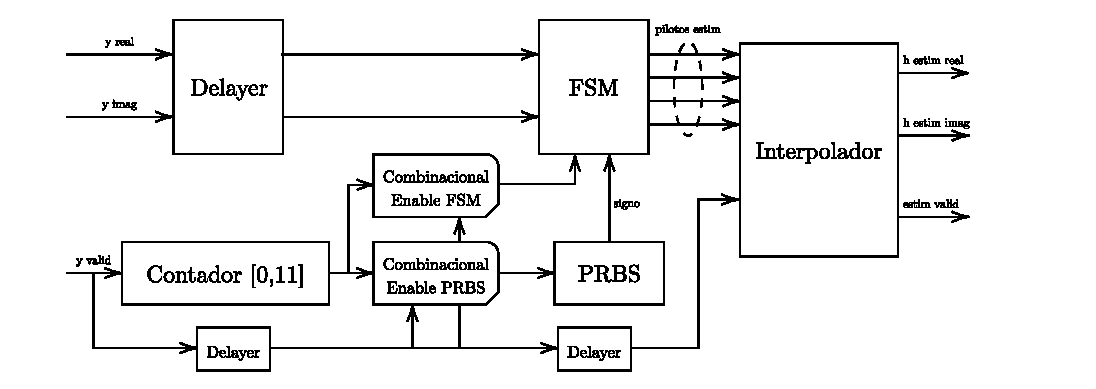
\includegraphics[width=1\columnwidth,trim={0 0 1cm 0},clip]{./Figures/Diagrama1.pdf} % Example image
		\captionof{figure}{Esquema del estimador del canal.}
	\end{center}
	\label{implementacion}
\end{minipage}

Merece la pena pararse a comentar algunos detalles del sistema que será de utilidad para la sección posterior, analizando en detalle los bloques. Las entradas del sistema, como en la propuesta, son los datos como números complejos y la señal bandera \emph{y\_valid} que indica cuando estos datos son nuevos. Aquí se encuentra una de las primeras (y principales) desventajas de trabajar con \emph{CoCoTb}, la cual es el no poder usar datos de tipo \emph{record}, lo cual aporta bastante limpieza y simplicidad al código, así que todas las señales que representen valores complejos estarán separadas en real e imaginaria.

Sobre el funcionamiento del sistema en conjunto, para empezar se asumirá, como en Matlab, que el primer piloto es la primera muestra del símbolo. La secuencia de datos comenzará a mover el sistema, haciendo que el contador tome el valor inicial 0, al estar cargado con el valor de \emph{reset} 11, de manera que piloto y valor del contador 0 vayan al unísono. Los circuitos combinacionales controlarán la señal de activación para los bloques FSM y PRBS, donde la segunda irá un ciclo de reloj por delante, para que el PRBS tenga tiempo a calcular el siguiente signo. En el bloque FSM se calculará la h estimada según $h_{estimada} = \pm Y$ dependiendo del valor del signo y por un proceso se asignarán los valores de los pilotos correspondientes. Para acabar, el bloque interpolador recibirá las señales h del bloque FSM en conjunto con el dato \emph{valid}, el cual avisará de cuando debe funcionar el bloque. Las salidas pues, serán estimación real e imaginaria del canal en ese ciclo y una bandera indicando si es un dato nuevo.

Los bloques \emph{Delayer} que se encuentran dispersos por la aquitectura del estimador sirven para compensar los retardos ocasionados por los circuitos no combinacionales, a parte de servir para asegurar en un caso de implementación real que los retardos en las puertas lógicas no afecten a nuestro circuito. 

% \begin{figure}[h] % [h] forces the figure to be output where it is defined in the code (it suppresses floating)
% 	\centering
% 	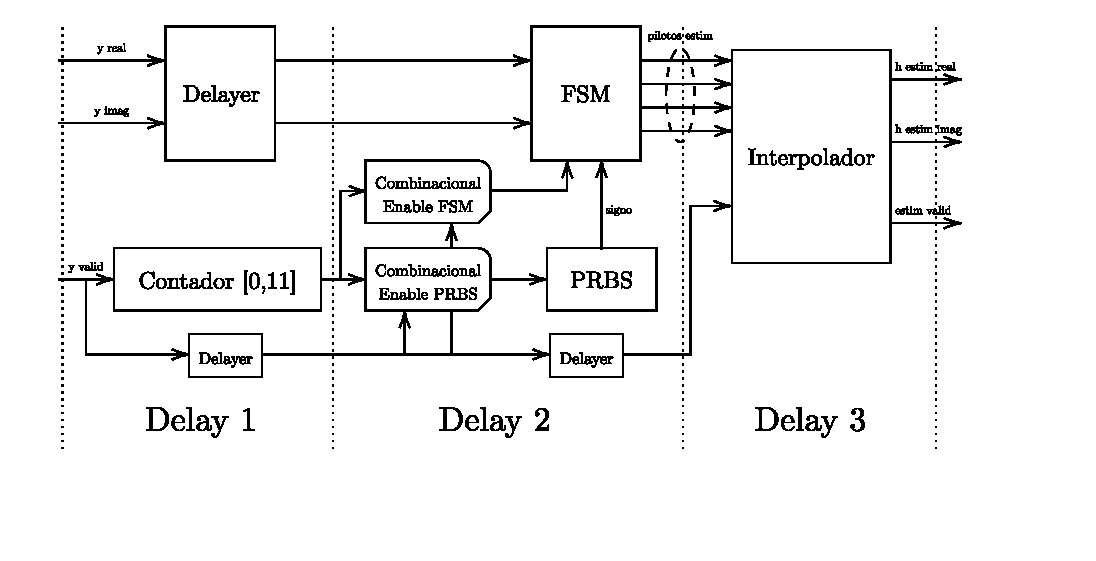
\includegraphics[width=1\columnwidth,trim={0 2cm 1cm 0},clip]{./Figures/DiagramaDelays.pdf} % Example image
% 	\caption{Retrasos del sistema.}
% 	\label{delays}
% \end{figure}

\begin{minipage}{\linewidth}
	\begin{center}
		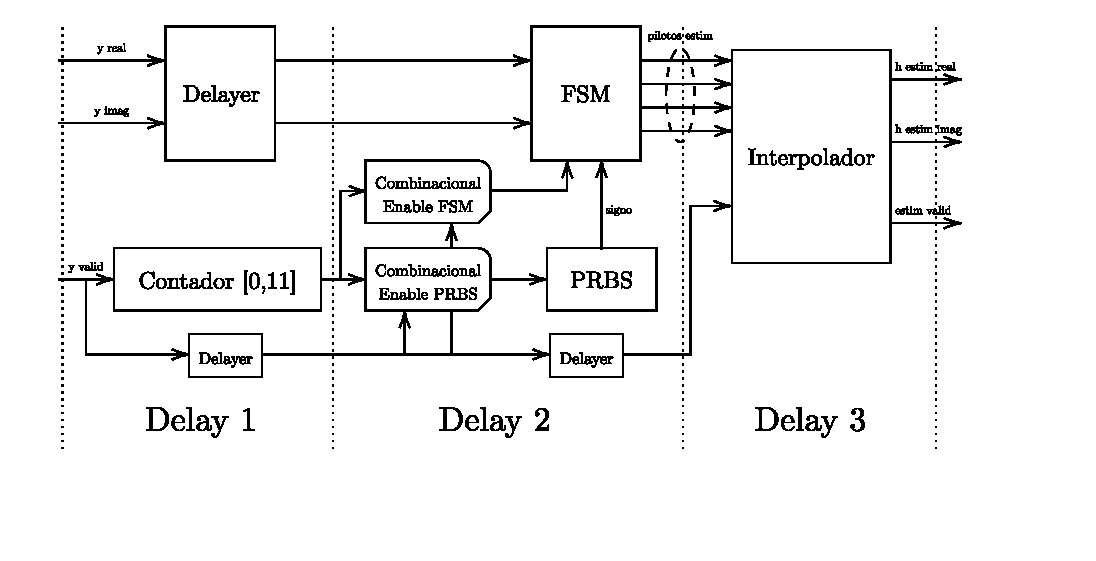
\includegraphics[width=1\columnwidth,trim={0 2cm 1cm 0},clip]{./Figures/DiagramaDelays.pdf} % Example image
	\captionof{figure}{Retrasos del sistema.}
	\end{center}
	\label{delays}
\end{minipage}

En la Figura \ref{delays} se muestra sobre el diagrama original como afectan los bloques síncronos al diseño. Como se ha comentado, al ser \emph{pipeline}, y con un flujo de datos constante, los valores de salida se procesarían continuamente y saldría con un retraso de tres periodos de reloj tras la entrada del primer dato. 

Para acabar, resta comentar el añadido del ecualizador. Este ha sido realizado mediante divisiones combinacionales para aprovechar la arquitecura en serie que se ha usado y continuar con la filosofía de trabajo de intentar mantenerlo lo más simple posible.

\begin{minipage}{\linewidth}
	\begin{center}
		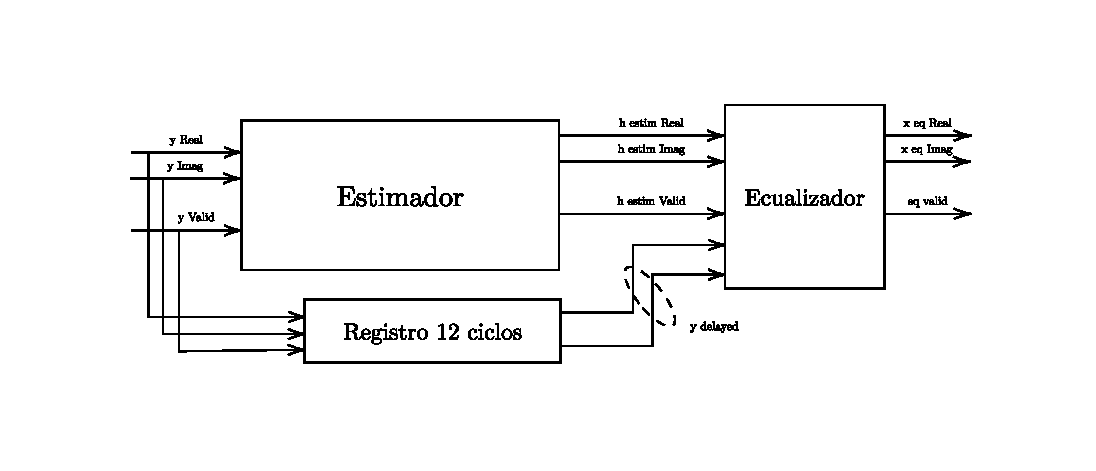
\includegraphics[width=1\columnwidth,trim={0 1cm 1cm 0},clip]{./Figures/diagrameq.pdf} % Example image
	\captionof{figure}{Sistema completo con ecualización.}
	\end{center}
	\label{ecualizador}
\end{minipage}

Lo más relevante que debe ser comentado sobre este diseño es el hecho de que las primeras 12 estimaciones del estimador de canal serán inútiles, ya que corresponden a una interpolación entre el primer piloto y el valor de \emph{reset}, por lo que los datos deben entrar en el ecualizador retrasados 12 ciclos debido a este hecho más los 3 que tarda en realizar sus procesos.

\Newpage

\section{Análisis de los códigos}

En esta sección se verán en detalle los códigos VHDL usados y los \emph{test benchs} para verificarlos uno a uno, dando enfásis en las partes más importantes. Para una mayor claridad, los códigos de VHDL estarán resaltados en azul y los de Python en negro.

\subsection{Contador}

El contador es un bloque muy simple, el cual contará de 0 a 11 para señalar cuando viene un piloto. Lo más interesante es el generic para controlar su valor de inicio, usado para poder en fase al contador con los pilotos. Es habilitado por la señal de dato válido.

\begin{minted}[linenos=true, bgcolor = colorVHDL, frame = single, breaklines = true]{vhdl}
entity contador1_12 is
	-- Generic defines beginning value for counter, in case is needed an uncommon start
	generic (
	start : integer := 11
	);
	port (
	rst    : in  std_logic;
	clk    : in  std_logic;
	ena    : in  std_logic;
	cuenta : out unsigned(3 downto 0)
	);
end contador1_12;
\end{minted}

En cuanto a su verificación, ha sido realizada una muy simple para comprobar su correcto funcionamiento. Aún así, es intersante echarle un ojo para comentar algunas bases de \emph{CoCoTb} que se usarán en muchos \emph{testbenchs}.

\begin{minted}[linenos = true, bgcolor = negro, frame = single]{python}
import cocotb
from cocotb.triggers import Timer
from cocotb.triggers import RisingEdge
import matplotlib.pyplot as plt
import numpy as np
# import oct2py
\end{minted}

Un ejemplo de las librerías que se usarán, donde destaca cocotb, que es la principal. Por otro lado está matplotlib.pyplot para gráficas, numpy para operar con vectores y oct2py para mover códigos matlab.

\begin{minted}[linenos = true, bgcolor = negro, frame = single]{python}
maxCycles = 120
currentCycle = 0

async def generate_clock(dut):
    """Generate clock pulses."""
    global maxCycles,currentCycle
    for cycle in range(maxCycles):
        dut.clk.value = 0
        await Timer(1, units="ns")
        dut.clk.value = 1
        await Timer(1, units="ns")
        currentCycle += 1
\end{minted}

Este trozo de código define variables globales para el número máximo de ciclos y el ciclo actual. Mientras tanto en la función se define el ciclo de reloj y se aumenta este valor de la variable para seguirla por todo el prograna.

\begin{minted}[linenos = true, bgcolor = negro, frame = single]{python}
@cocotb.test()
async def test1(dut):
    global maxCycles,currentCycle
    values = []
    await cocotb.start(generate_clock(dut))

    dut.rst.value = 1

    await RisingEdge(dut.clk)

    dut.ena.value = 1
    dut.rst.value = 0

    while currentCycle < maxCycles-1:
        await RisingEdge(dut.clk)
        values.append(int(dut.cuenta))

    print(values)
\end{minted}

Para acabar el test en sí, primero se definen las variables, se le da el reset y se deja aumentar el clk con la sentencia Await RisingEdge. Este será el bucle principal del \emph{testbench}, donde se tocará la mayor parte de las cosas. 

\subsection{Delayer}

Este bloque también es muy sencillo pero merece comentarse aún así. Ha sido verificado con gtkwave en conjunto con el estimador por lo que no se muestra su \emph{test bench} aquí. Su funcionamiento se basa en generar biestables para todos los bits de los datos y dárselos de entrada al bloque FSM.

\subsection{PRBS}

Bloque para la generación del código pseudo aleatorio para los pilotos. Es bastante directo hacer este bloque partiendo del contador. Algunos detalles interesantes son: el bloque principal, donde hubo problemas de compilación al no especificar a ghdl mediante el makefile de CoCoTb la versión del VHDL deseada.

\begin{minted}[linenos=true, bgcolor = colorVHDL, frame = single, breaklines = true]{vhdl}
process (reg)
begin
	-- not working till GHDL_ARGS ?= --std=08 is used in GHDL compiler from cocotb (thanks to @hipolitoguzman)
	preg <= (11 downto 2 => reg(10 downto 1), 1 => reg(11) xor reg(9));
	
	-- workaround
	-- preg(11 downto 2) <= reg(10 downto 1);
	-- preg(1) <= reg(11) xor reg(9);
end process;
\end{minted}

También es interesante el valor de inicio del PRBS, el cual no coincide con el dicho en el estándar, que es todo 1's. Esta inicialización es así debido a que es necesario retrasar los signos del PRBS un ciclo, y así se consigue sin modificar la secuencia futura, consiguiendo que sea totalmente compatible con un sistema DVBT.

\begin{minted}[linenos=true, bgcolor = colorVHDL, frame = single, breaklines = true]{vhdl}
process (clk,rst)
begin
	if rst = '1' then
	-- indexin n slicin
	reg <= (11 => '0',10 => '1', others => '1');
	elsif rising_edge(clk) then
	if ena = '1' then
		reg <= preg;
	else
		reg <= reg;
	end if;
	end if;
end process;
\end{minted}

En un principio se tuvo en cuenta que el PRBS solo se activaba cada doce ciclos, cuando no es así. Esto fue fácilmente modificado para respetar el estándar cambiando el bloque combinacional de habilitación del PRBS, dependiendo directamente del dato válido y no del contador.

Respecto al \emph{testbench}, se han realizado dos, uno muy básico para ver los signos, y otro más interesante en el cual se usa la librería oct2py para comparar con el código Matlab.

\begin{minted}[linenos=true, bgcolor = negro, frame = single, breaklines = true]{python}
from oct2py import octave
goldenSignos = octave.PRBS(1,1705)
goldenSignos = (goldenSignos[0,:]+1)/2
# dut._log.info(signos)
dut._log.info(goldenSignos.shape)
# print(goldenSignos.shape)

plt.subplot(211)
plt.stem(signos)
plt.subplot(212)
plt.stem(goldenSignos)
plt.show()
\end{minted}

Llama la atención como se accede fácilmente a la función previamente definida PRBS.m, como se tratan los datos y los plots. Además se usa dut.\_log.info para escribir en el logger con el nivel de altera "info".

\begin{minipage}{\linewidth}
	\begin{center}
		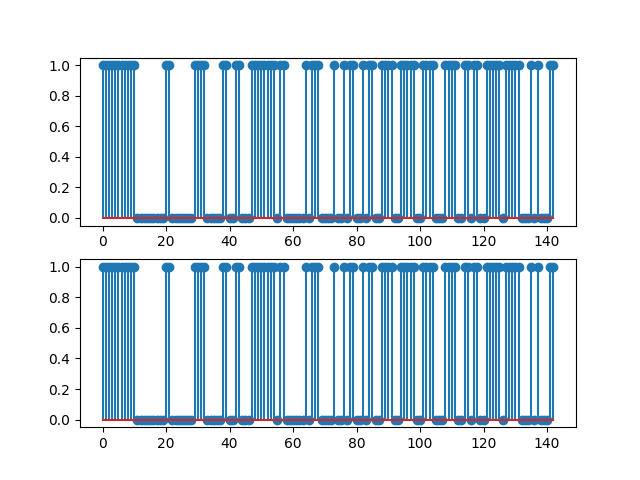
\includegraphics[width=1\columnwidth,trim={0 0.5cm 1cm 1cm},clip]{../../Linux/P2/CoCoTb/pilotos.png} % Example image
	\captionof{figure}{Pilotos Matlab vs VHDL.}
	\end{center}
	\label{pilotos}
\end{minipage}

\subsection{FSM}

El bloque FSM se llama así por que en las primeras etapas del diseño del funcionamiento del sistema iba a ser una máquina de estados, pero al final se consiguió simplificar tanto que se convirtió en un circuito síncrono sin estados, y conservó ese nombre como bloque. Su función es la de recibir los pilotos y el signo del generador PRBS para así estimar el valor de h. Para esta función deberá, cada vez que venga un piloto, cambiar el piloto servido como superior al interpolador por el inferior y añadir el nuevo que llega como inferior.

Básicamente es un circuito síncrono que se encarga de cuando le llega la señal \emph{write\_enable} cambiar los valores de las h estimadas superior e inferior, cambiandoles el signo si es necesario según el valor del signo arrojado por el bloque PRBS.

\begin{minted}[linenos=true, bgcolor = colorVHDL, frame = single, breaklines = true]{vhdl}
-- changing sign depending on PRBS
if PRBS = '1' then
	p_h_sup_re <= piloto_y_re;
	p_h_sup_im <= piloto_y_im;
	p_h_inf_re <= h_sup_re;
	p_h_inf_im <= h_sup_im;
else
	p_h_sup_re <= -piloto_y_re;
	p_h_sup_im <= -piloto_y_im;
	p_h_inf_re <= h_sup_re;
	p_h_inf_im <= h_sup_im;
end if;
\end{minted}

Por dentro tiene poca lógica, solo destacar el if decidiendo como cambia el signo de los pilotos según el valor del PRBS. El resto del código es un circuito síncrono común.

En verificación se ha estudiado si realmente obtiene los pilotos en el momento correcto y no en cualquier otro. Para esto se ha pasado el valor de entrada 69 en todos los instantes incorrectos, mientras que en los slots de los pilotos se pasa $10 + i*5$ para la parte real y $100 + i*10$ a la imaginaria para comprobar que correctamente aumentan los valores, es decir, cambian cada doce ciclos.

Si por alguna razón toma valores incorrectos, es decir, 69, salta una excpeción. 

\begin{minted}[linenos=true, bgcolor = negro, frame = single, breaklines = true]{python}
# try avoids int(XXX) or int(uuu) case
# this could be avoided by cocotb's 
# resolve u, which would change u bit values to
# one at our choice, but we would lose some sight of 
# what is happening.
try:
	int(dut.inf_re.value)
	int(dut.inf_im.value)
	int(dut.sup_re.value)
	int(dut.sup_im.value)
except:
	pass
else:
	# if pilots values are correctly casted into int, check if they got wrong values (samples values are represented by 69)
	if dut.inf_re.value == 69 or dut.inf_im.value == 69 or dut.sup_re.value == 69 or dut.sup_im.value == 69:        
		raise "El valor incorrecto ha sido propagaddo!"
\end{minted}

Aquí ya hay varios temas interesantes. Para empezar el la estructura try -> except -> else, sobretodo para realizar posteriormente el "try trick" que se explicará luego. Si el valor de los pilotos es incorrecto, salta la excepción.

Es uno de los primeros \emph{testbenchs} donde todavía estaba aprendiendo a manejarme, un tema importante es que si quieres pasar las variables de vhdl a python y en vhdl valen U o X habrá problemas graves. CoCoTb puede resolver automaticamente estos valores a 0 o 1, pero eso le restaría algo de fiabilidad a las verificaciones así que decidí ignorarlo.

\subsection{Interpolador}

Este bloque es el original que fue aportado para el trabajo de la asignatura pero \textbf{no} es el usado finalmente para la implementación, pero se proporciona también al haber realizado una verificación de este.

La verificación es bastante interesante ya que ha sido realizado un \emph{test bench} que contrasta contra datos generados aleatoriamene usando una arquitectura \emph{self-checking}. Estos datos posteriormente se grafican para ser comparados.

\begin{minted}[linenos=true, bgcolor = negro, frame = single, breaklines = true]{python}
inf_re = int(np.round((np.random.rand())*2**9))
inf_im = int(np.round((np.random.rand())*2**9))
sup_re = int(np.round((np.random.rand())*2**9))
sup_im = int(np.round((np.random.rand())*2**9))
\end{minted}

Así se generan fácilmente valores aleatorios como entradas. Para comparar si interpola bien en este caso se ha comparado con un predictor hecho en Python y no en matlab para mostrar la amplia gama de opciones a la hora de comprobar el funcionamiento del circuito, aunque aquí no se exploren demasiadas hay muchas más.

\begin{minipage}{\linewidth}
	\begin{center}
		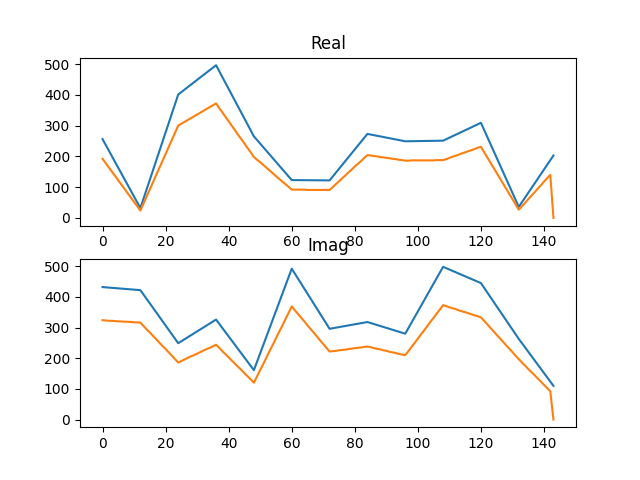
\includegraphics[width=1\columnwidth,trim={0 0.5cm 1cm 0.5cm},clip]{../../Linux/Trabajo/InterpoladorCCTb/imgs/interpolador_real_imag_sub_rand_superpuestas.png} % Example image
	\captionof{figure}{Interpolación Python vs VHDL.}
	\end{center}
	\label{interpolate}
\end{minipage}

Se puede ver como las formas de onda aleatorias son exactamente iguales pero ligeramente escalada una respecto a otra.

\subsection{InterMig}

Este es el interpolador que se usó finalmente para el proyecto. Se modificó para que cumpliera dos requisitos fundamentales, uno de ellos que tardara menos en interpolar, ya que el proporcionado tardaba trece por cada doce datos, lo cual arruinaba la arquitectura \emph{pipeline}, mientras que el otro requisito fue el que la señal valid tuviera que estar valiendo 1 en cada ciclo para que la interpolación se realizara. Esto último es debido a que si en algún momento dejaran de entrar datos, todo el sistema debe pararse a la vez, si la interpolación siguiera habría incompatibilidad entre partes. Los cambios realizados son pequeños y dispersos por lo que no se mostrará nada en concreto del código VHDL. Los objetivos nombrados se lograron cambiando el \emph{reset} y la señal de dato válido.

En el \emph{testbench} correspondiente, el cual es una modificación de la primera versión del interpolador original, se realizan dos tests en un mismoa archivo por primera vez en la memoria, lo cual se comentará luego, además de que se prueba el reset.

\subsection{AllButInterpolator}

Este código implementa todo los bloques menos el interpolador para comprobar que en conjunto todo va bien. Hubo un momento en el que las cosas fallaban y se comprobó el funcionamiento de los subbloques poco a poco para asegurar. Detalles intersantes de este bloque también se ven en TopLevel, así que se dejarán para esa parte al ser más improtante.

Las pruebas de este bloque fueron muy sencillas, solo para comprobar sus correctas conexiones. \emph{Testbench} también basado en el del interpolador original.

\subsection{TopLevel (Estimador)}

Esta unidad se encarga de conectar los anteriores bloques de la forma descrita en el primer apartado para lograr su correcto funcionamiento. Se define también como un proceso síncrono el retraso de la señal de dato válido para ser utilizado en otros bloques. Aquí se ven las sentencias que sintetizarían los bloques de habilitación de FSM y PRBS:

\begin{minted}[linenos=true, bgcolor = colorVHDL, frame = single, breaklines = true]{vhdl}
-- adding "and y_valid_delayed" becouse if we stop and cuenta value is 11 we get many prbs
-- enaPRBS <=  '1' when (cuenta_value = "1011" and y_valid_delayed_1 = '1')  else '0';
-- hpgm didnt like PRBS the way i did it, fixed
enaPRBS <=  '1' when (y_valid_delayed_1 = '1')  else '0';

-- same with FSM
enaFSM <=  '1' when (cuenta_value = "0000" and y_valid_delayed_2 = '1') else '0';
\end{minted}

Se cambió aquí el comentado error en el PRBS. También se tiene en cuenta el valor de dato válido y no solo el del contador para la problmática descrita en el comentario, cuando el sistema para y el contador se queda parado en cierto valor conflictivo (en su momento 0000 o 1111, después del cambio del PRBS solo 0000).

En cuanto al \emph{test bench}, se realizan varios tests, uno incial general, otro para comprobar el \emph{reset}, y los siguientes para los modos 2k y 8k. Para seleccionar cuales se quieren usar se hace uso de las variables globales skipn, de la siguiente forma:

\begin{minted}[linenos=true, bgcolor = negro, frame = single, breaklines = true]{python}
skip1 = True
skip2 = True
skip3 = False
skip4 = True

@cocotb.test(skip = skip1)
async def testIfWorks(dut):
	...
\end{minted}

Dando el valor False para ejecutar (no skip) y true para no ejecutar (skip). Adicionalmente, se define la función \emph{fromsigned2int} para recuperar los datos en formato signed20 a los integer de Python. Luego, al ver largos tiempos de computación se buscaron alternativas para agilizar el cómputo, llegando a la función versión 2, que reduce a más de la mitad el tiempo de procesado.

\begin{minted}[linenos=true, bgcolor = negro, frame = single, breaklines = true]{python}
def fromsigned2int(bits,base):
    v = base**np.arange(bits.shape[1],0,-1)
    v[0] = -v[0]
    return np.sum(bits*np.kron(np.ones((bits.shape[0],1)),v),axis=1)

# much much faster (halves time to compute)
def fromsigned2intv2(bits):
    return np.array([value.signed_integer for value in bits])
\end{minted}

Otro detalle es el hecho de usar cierta configuración de matplotlib.pyplot usada para el modo \emph{headless}, esto será útil para la integración continua con Docker, acelerando el computo al no necesitar mostrar la gráfica. Esta opción se activa así:

\begin{minted}[linenos=true, bgcolor = negro, frame = single, breaklines = true]{python}
import matplotlib
matplotlib.use('Agg')
\end{minted}

La estrucutra en sí del \emph{testbench} es muy interesante, destacando el uso de octave.addpath para añadir la carpeta de los códicos Octave al directorio de trabajo y el escalado de las muestras.

Para acabar, algunas gráficas arrojadas por el programa:

\begin{minipage}{\linewidth}
	\begin{center}
		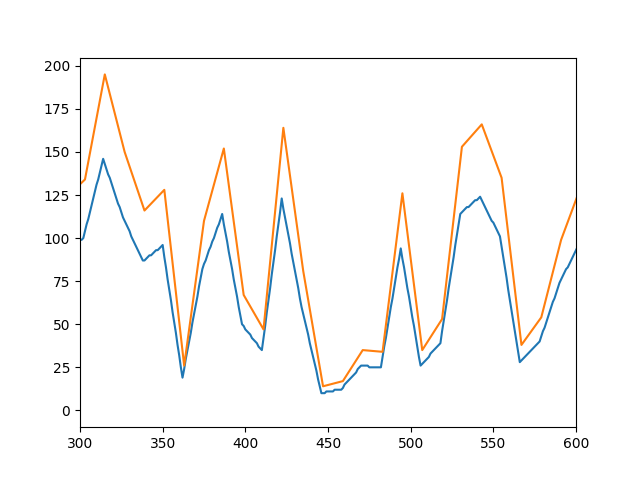
\includegraphics[width=1\columnwidth,trim={0 0.5cm 1cm 0.5cm},clip]{../../Linux/Trabajo/TopLevelCCTb/imgs/pilotos.png} % Example image
	\captionof{figure}{Interpolación Python vs VHDL.}
	\end{center}
	\label{pilotosveriftoplevel}
\end{minipage}

Aquí se puede ver como los pilotos en conjunto con todo el circuito funcionan bien. Pasando a interpolación está el modo 2k:

\begin{minipage}{\linewidth}
	\begin{center}
		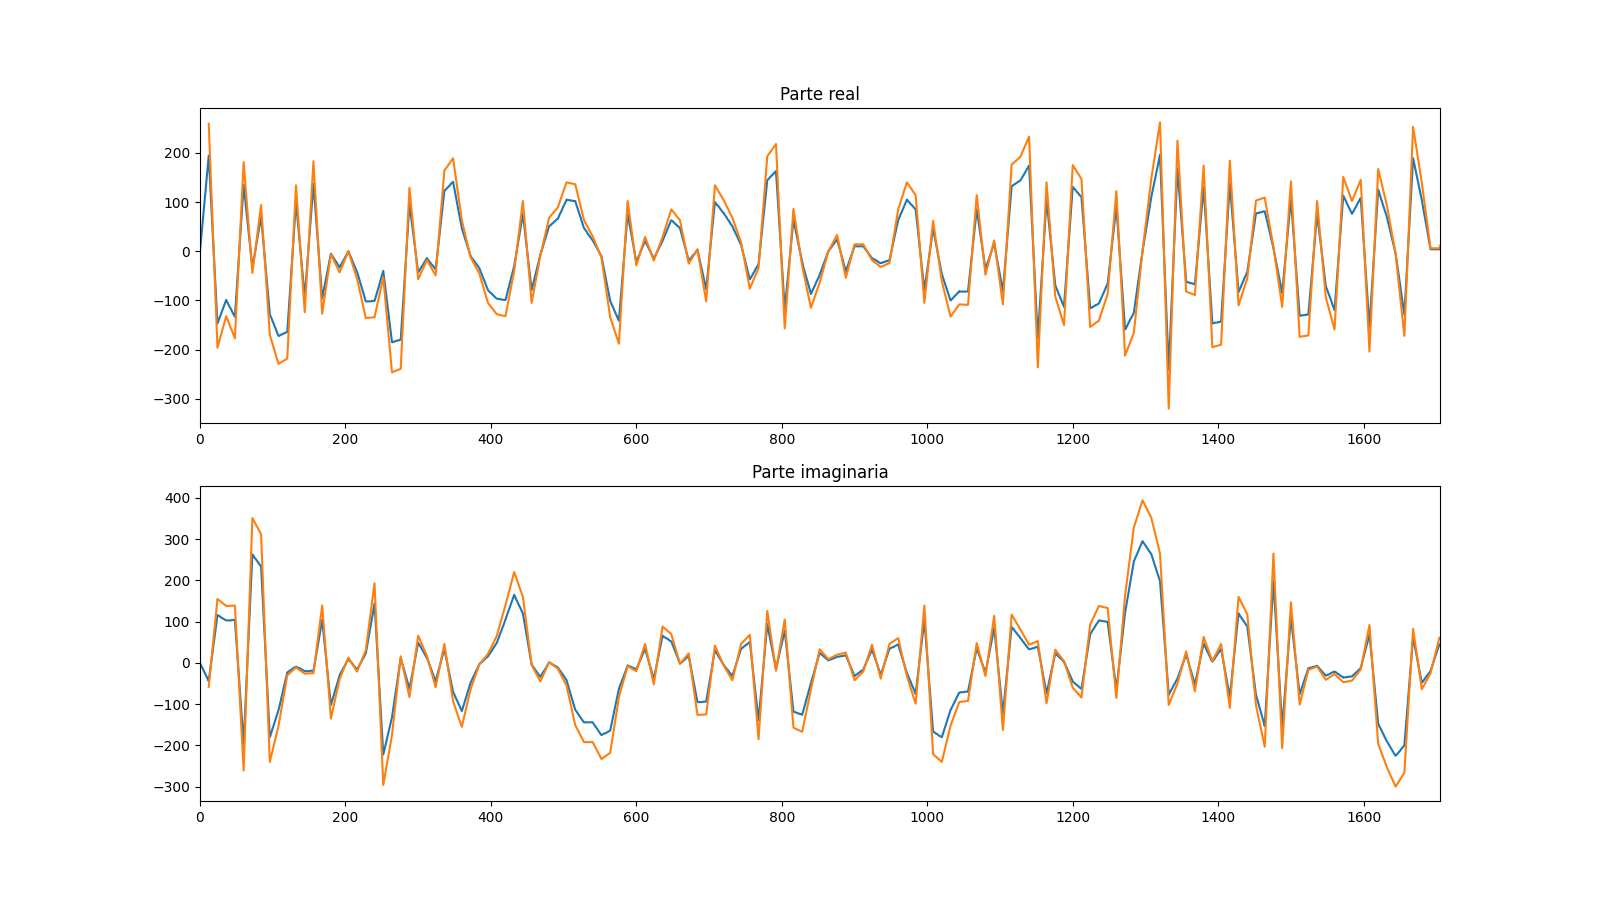
\includegraphics[width=1\columnwidth,trim={0 0.5cm 1cm 0.5cm},clip]{../../Linux/Trabajo/TopLevelCCTb/imgs/vsOctave2.png} % Example image
	\captionof{figure}{Estimación Matlab vs VHDL modo 2k.}
	\end{center}
	\label{modo2kestimar}
\end{minipage}

Y en el modo 8k:

\begin{minipage}{\linewidth}
	\begin{center}
		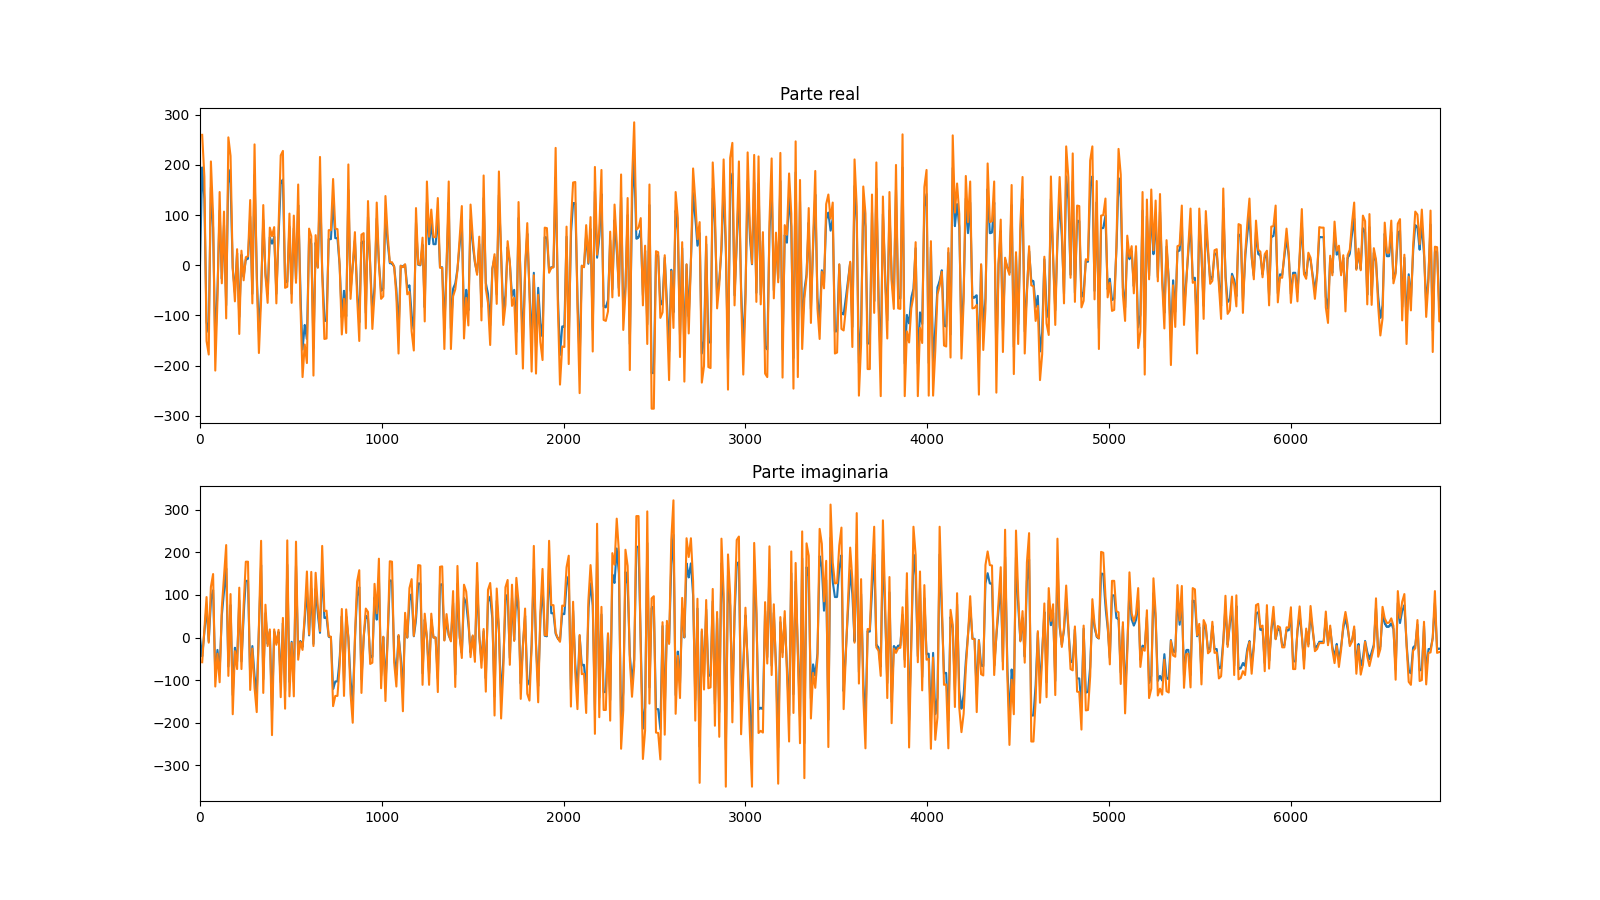
\includegraphics[width=1\columnwidth,trim={0 0.5cm 1cm 0.5cm},clip]{../../Linux/Trabajo/TopLevelCCTb/imgs/vsOctave8.png} % Example image
	\captionof{figure}{Estimación Matlab vs VHDL modo 8k.}
	\end{center}
	\label{modo8kestimar}
\end{minipage}

\subsection{Ecualizador}

El bloque final es el equalizador de canal, el cual se encarga de dividir las muestras $y$ entre el canal estimado $h$ para revertir los efectos del canal. Esta operación se ha propuesto como un circuito combinacional, haciendo uso del operador $\backslash$ para realizar la división combinacional, lo cual consume mucha área pero permite que el diseño conserve su estructura \emph{pipeline}. También habría que, en el diseño real, fijarse en el tiempo que tardan todas esas puertas lógicas en realizar las operaciones, pero al ser simulación funcionará, por lo que en una implementacion se dejaría la comprobación del correcto funcionamiento físico. Los resultados se escalan por $2^{10}$ gracias a un desplazamientopara realizar la división. Este factor de escala luego se corrije.

La división y multiplicación está definida según la multipliación compleja

\begin{equation} 
	% \label{eq1}
	\begin{split}
		(a + j b) (c +j d) &= (e + j f) \\
						e  &= a c + b d	\\
						f  &= b c - a d
	\end{split}
\end{equation}

Posteriormente este valor se dividirá entre el módulo de la h estimada.

El \emph{test bench} del bloque es extremadamente sencillo, ya que se simulará posteriormente en conjunto con todo el sistema, así que solo se realizaron comprobaciones leves.

\subsection{Registro}

A parte del ecualizador otro bloque más será necesario para el correcto funcionamiento de todo el sistema. Como se comentó al principio, entre los doce ciclos que hay que esperar para que el interpoladro arroje valores válidos y los tres ciclos de reloj de retardo, la señal $y$ de entrada al ecualizador tendrá que retrasarse, eso es lo que hará este bloque.

Lo más importante en mi opnión es la definición del tipo array para crear el registro, de esta manera:

\begin{minted}[linenos=true, bgcolor = colorVHDL, frame = single, breaklines = true]{vhdl}
type reg is array (0 to delay-1) of signed(9 downto 0);
signal p_regis,regis : reg := (others => (others => '0'));
\end{minted}

Para verificar el registro se generan valores enteros incrementando a cada ciclo su valor en 1 unidad, para comprobar en gtkwave que los valores avanzan correctamente por el registro.

\subsection{Sistema completo}

Este último código tiene de tarea fundamental unificar todos los bloques, dando lugar al sistema por completo. Solamente instancia el estimador, el cual reunía todos los demás bloques, el ecualizador y el registro. 

Es un código bastante limpio ya que solo instancia componentes, conectándolos entre ellos.

En cuanto a verificar, se realizan cinco \emph{tests} de forma similar al estimador, uno inicial, otro del reset, un modo 2k contra un canal plano y posteriormente para los modos 2k y 8k, otra vez contra Matlab, todo bajo el \emph{engine} de Octave.

Para empezar, se usarán varias figuras de mérito:

\begin{minted}[linenos=true, bgcolor = negro, frame = single, breaklines = true]{python}
def MSE(x,y):
    return 10*np.log10((norm(x-y)/len(x)))

# using norm instead of mean square
def RMSE(x,y):
    return 10*np.log10(np.sqrt((norm(((x-y)))/len(x))))

def MAE(x,y):
    return np.mean(np.abs(x-y))
\end{minted}
	
Las figuras serán usadas con sus argumentos normalizados, MSE y RMSE serán encargadas de medir el parecido de las señales de salida mientras que el MAE calculará el error absoluto.

En el primer test se generan datos aleatorios. No hay nada muy importante que comentar del código pero será la base de los siguientes puesto que integra muchas cosas pequeñas que en conjunto logran un test robusto.

En el primer test se ecualiza en un canal plano con datos aleatorios. Los resultados son muy cercanos a ser perfectos, donde se obtienen unos resultados muy buenos:

\vspace{5mm}

\begin{minipage}{\linewidth}
	\begin{center}
	% \begin{table}[h] % [h] forces the table to be output where it is defined in the code (it suppresses floating)
	\centering % Centre the table
		\begin{tabular}{l l l l}
		\toprule
		\textit{M.F.} & \textbf{MSE [dB]} & \textbf{RMSE [dB]} & \textbf{MAE}\\
		\midrule
		Real & $-\inf$ &  $-\inf$ & $ 0 $ \\
		Imag & $-185.6$ &  $-92.8$ & $6 \cdot 10^{-18}$ \\
		Complex & $-188.6$ &  $-94.3$ & $3 \cdot 10^{-18}$ \\
		\bottomrule
	\end{tabular}
	% \caption{Sausage nutrition.}
	% \end{table}
	\captionof{table}{Resultados con datos aleatorios canal plano.}
	\end{center}
	% \label{tablaflatrandom}
\end{minipage}

\begin{minipage}{\linewidth}
	\begin{center}
		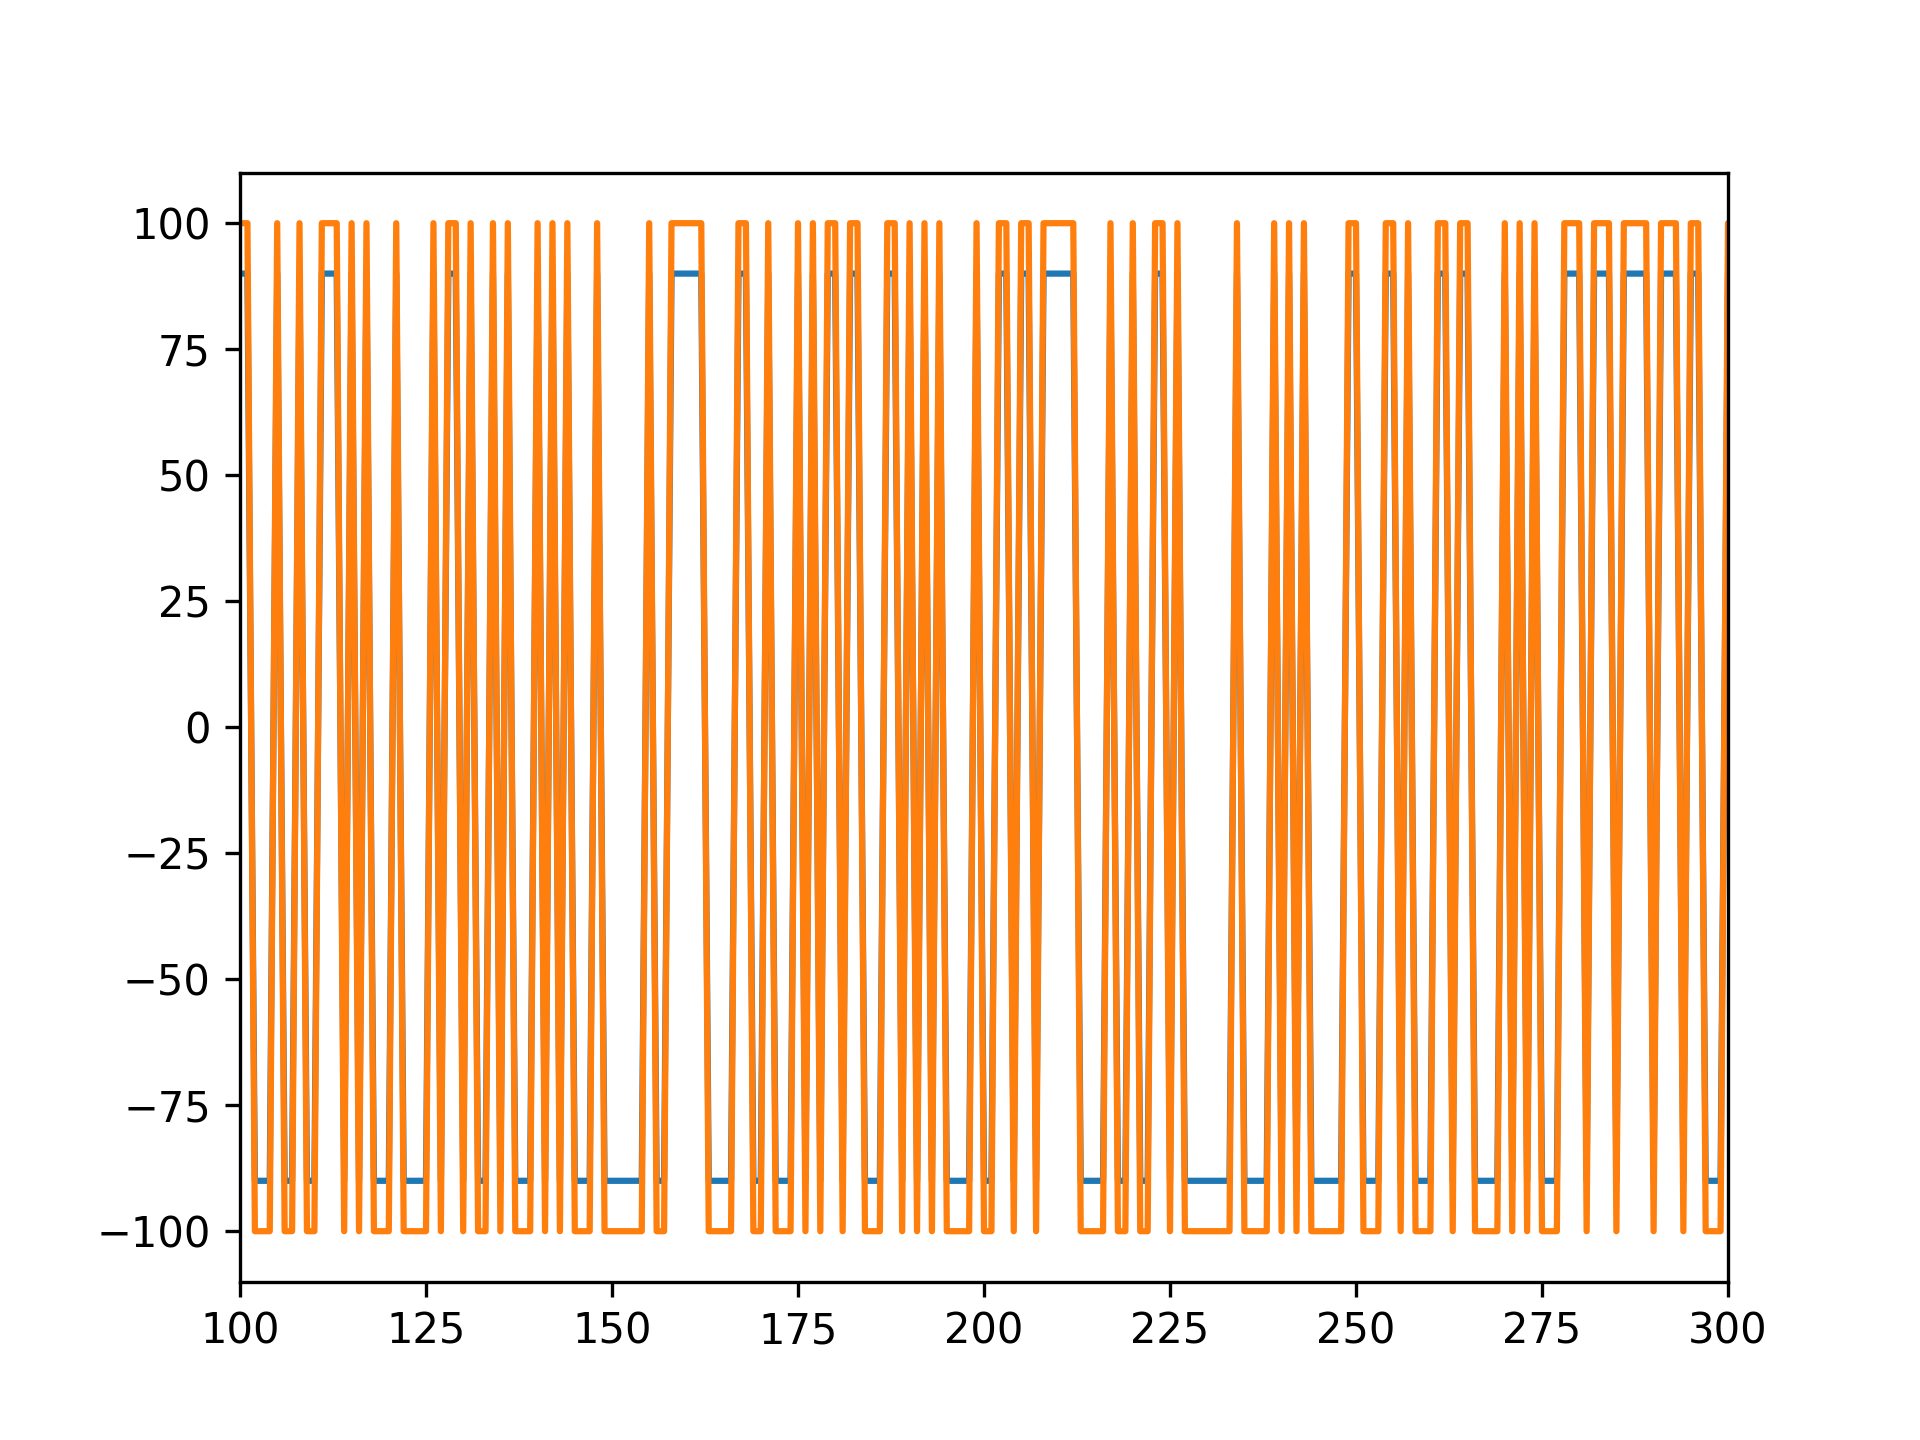
\includegraphics[width=1\columnwidth,trim={0 0.5cm 1cm 1cm},clip]{../../Linux/Trabajo/FullSystemCCTb/imgs/eq.png} % Example image
	\captionof{figure}{Ecualización con datos aleatorios canal plano, parte real.}
	\end{center}
	\label{eqrandomflat}
\end{minipage}

En esta última figura se muestra los datos ecualizados contra Matlab y la estimación del canal. Los datos equalizados están normalizados, y a la salida del VHDL, en azul, se le ha aplicado un pequeño factor de escala para verla bien con respecto a la de Matlab.

Por otro lado está el \emph{test} del reset que hace una comprobación muy simple. Este test se ha implementado anteriormente, simplemente para asegurar su correcto reinicio. Se genera un canal aleatorio para su comporbación.

Pasando directamente al tercero, que ya es más interesante, donde se compara contra Matlab sin introducir canal, a ver que tal es el rendimiento. En este caso se usa un símbolo 2k y se prueban distintas modulaciones. 

Es bastante interesante ya que trabaja con el archivo de Matlab, aprovechando la parametrización, desactivando el canal y creando un caso ideal.

Otra vez es un código que se apoya mucho en los anteriores, donde lo más relevante es la inclusión de una excpeción para fallar el test en el caso de que los resultados no sean los esperados. En este caso se ha fijado -20dB de MSE, un valor aceptable. Esta variable se incluirá en los demás, tanto de canal DVBT con o sin ruido para avisar cuando se haga CI de si algo se ha roto.

\begin{minted}[linenos=true, bgcolor = negro, frame = single, breaklines = true]{python}
if MSEcomplex >= -20:
	raise NameError("El error es mayor que el límite establecido, %d > -20 dB" % MSEcomplex)
\end{minted}

\vspace{5mm}
\begin{minipage}{\linewidth}
	\begin{center}
	% \begin{table}[h] % [h] forces the table to be output where it is defined in the code (it suppresses floating)
	\centering % Centre the table
		\begin{tabular}{l l l l}
		\toprule
		\textit{M.F.} & \textbf{MSE [dB]} & \textbf{RMSE [dB]} & \textbf{MAE}\\
		\midrule
		BPSK & $-59.5$ &  $-29.7$ & $4.3 \cdot 10^{-5}$ \\
		QPSK & $-61$ &  $-30.5$ & $2.25 \cdot 10^{-5}$ \\
		16QAM & $-61$ &  $-29.7$ & $2.3 \cdot 10^{-5}$ \\
		\bottomrule
	\end{tabular}
	% \caption{Sausage nutrition.}
	% \end{table}
	\captionof{table}{Resultados canal plano contra Matlab de señales complejas.}
	\end{center}
	% \label{tablaflatmatlab}
\end{minipage}

Hay una interesate interración y es que si el canal es absolutamente plano, en ausencia de ruido y la parte real o imaginaria valen cero, caso que se cumple para BPSK, canal plano y sin ruido, el sistema diverge al estimar el canal, por lo que se les ha añadido ruido a todos los experimentos de la tabla para hacerlo más justo, $SNR = 60$. Se puede ver como aún así, el error sale en la BPSK algo peor.

\begin{minipage}{\linewidth}
	\begin{center}
		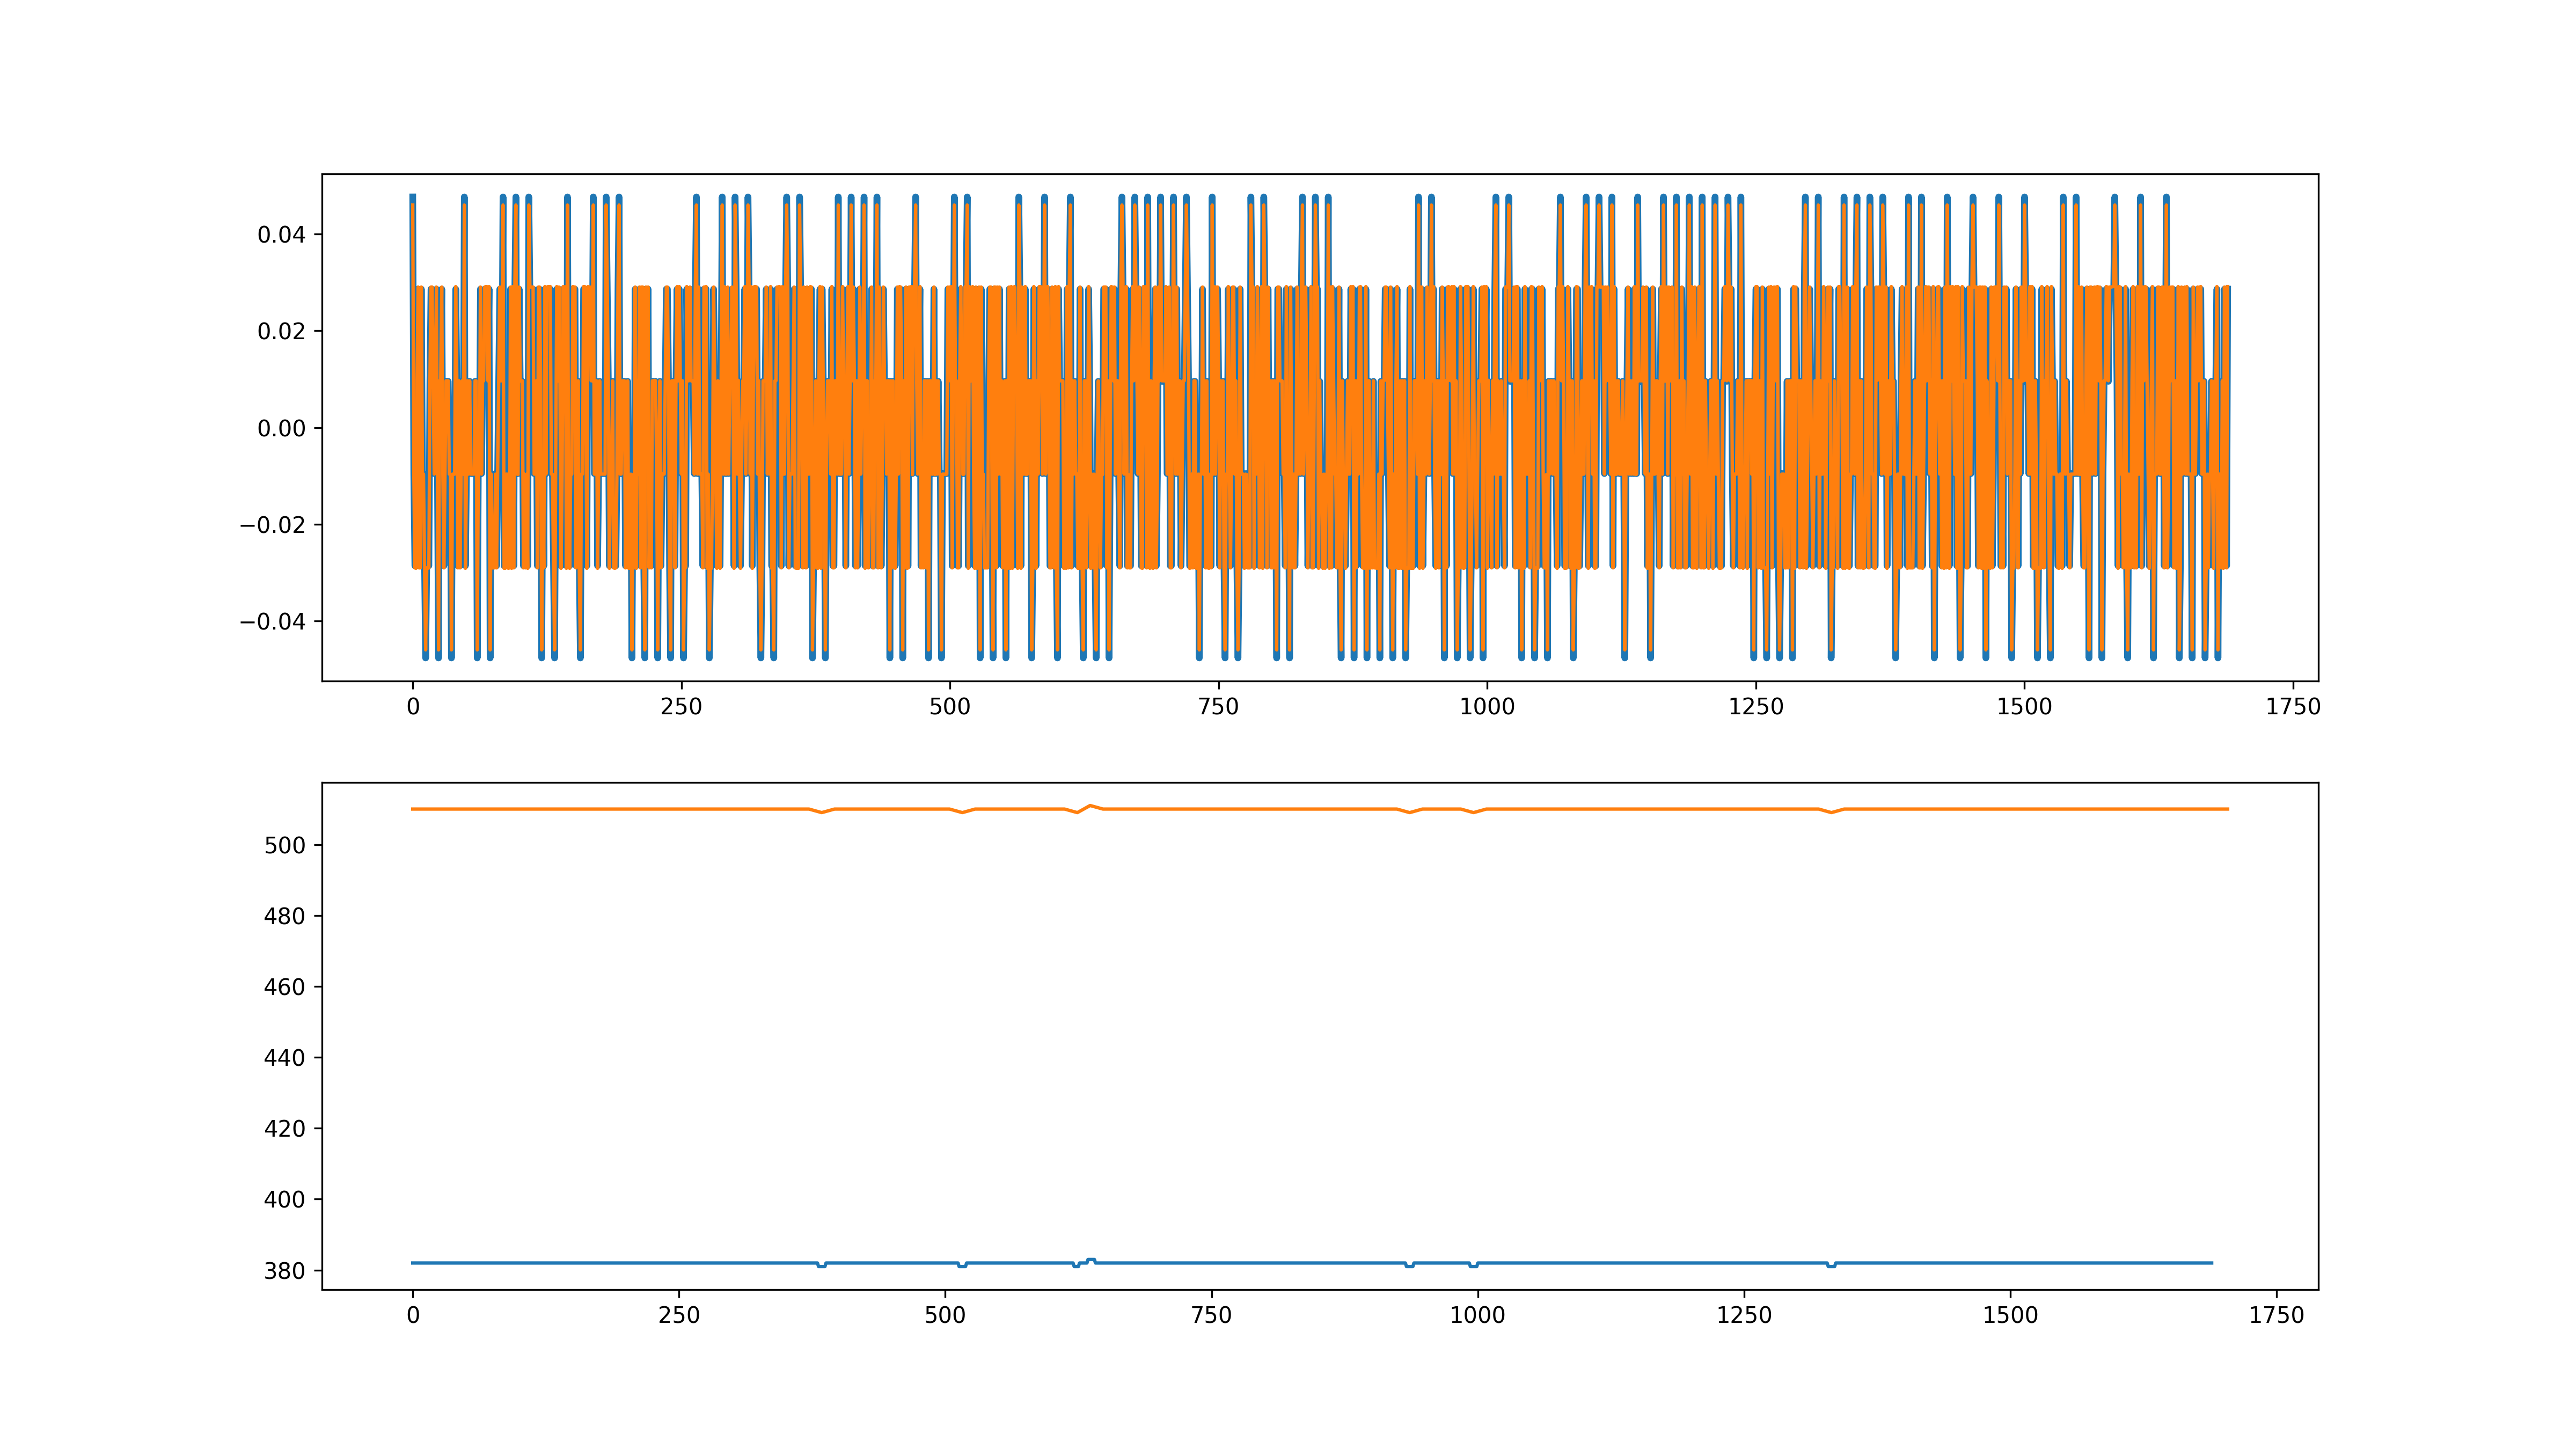
\includegraphics[width=1\columnwidth,trim={0 0.5cm 1cm 1cm},clip]{../../Linux/Trabajo/FullSystemCCTb/imgs/vsOctave2flatre.png} % Example image
	\captionof{figure}{Ecualización contra Matlab 16QAM con ruido, parte real.}
	\end{center}
	\label{eqmatlabflatre}
\end{minipage}	

\begin{minipage}{\linewidth}
	\begin{center}
		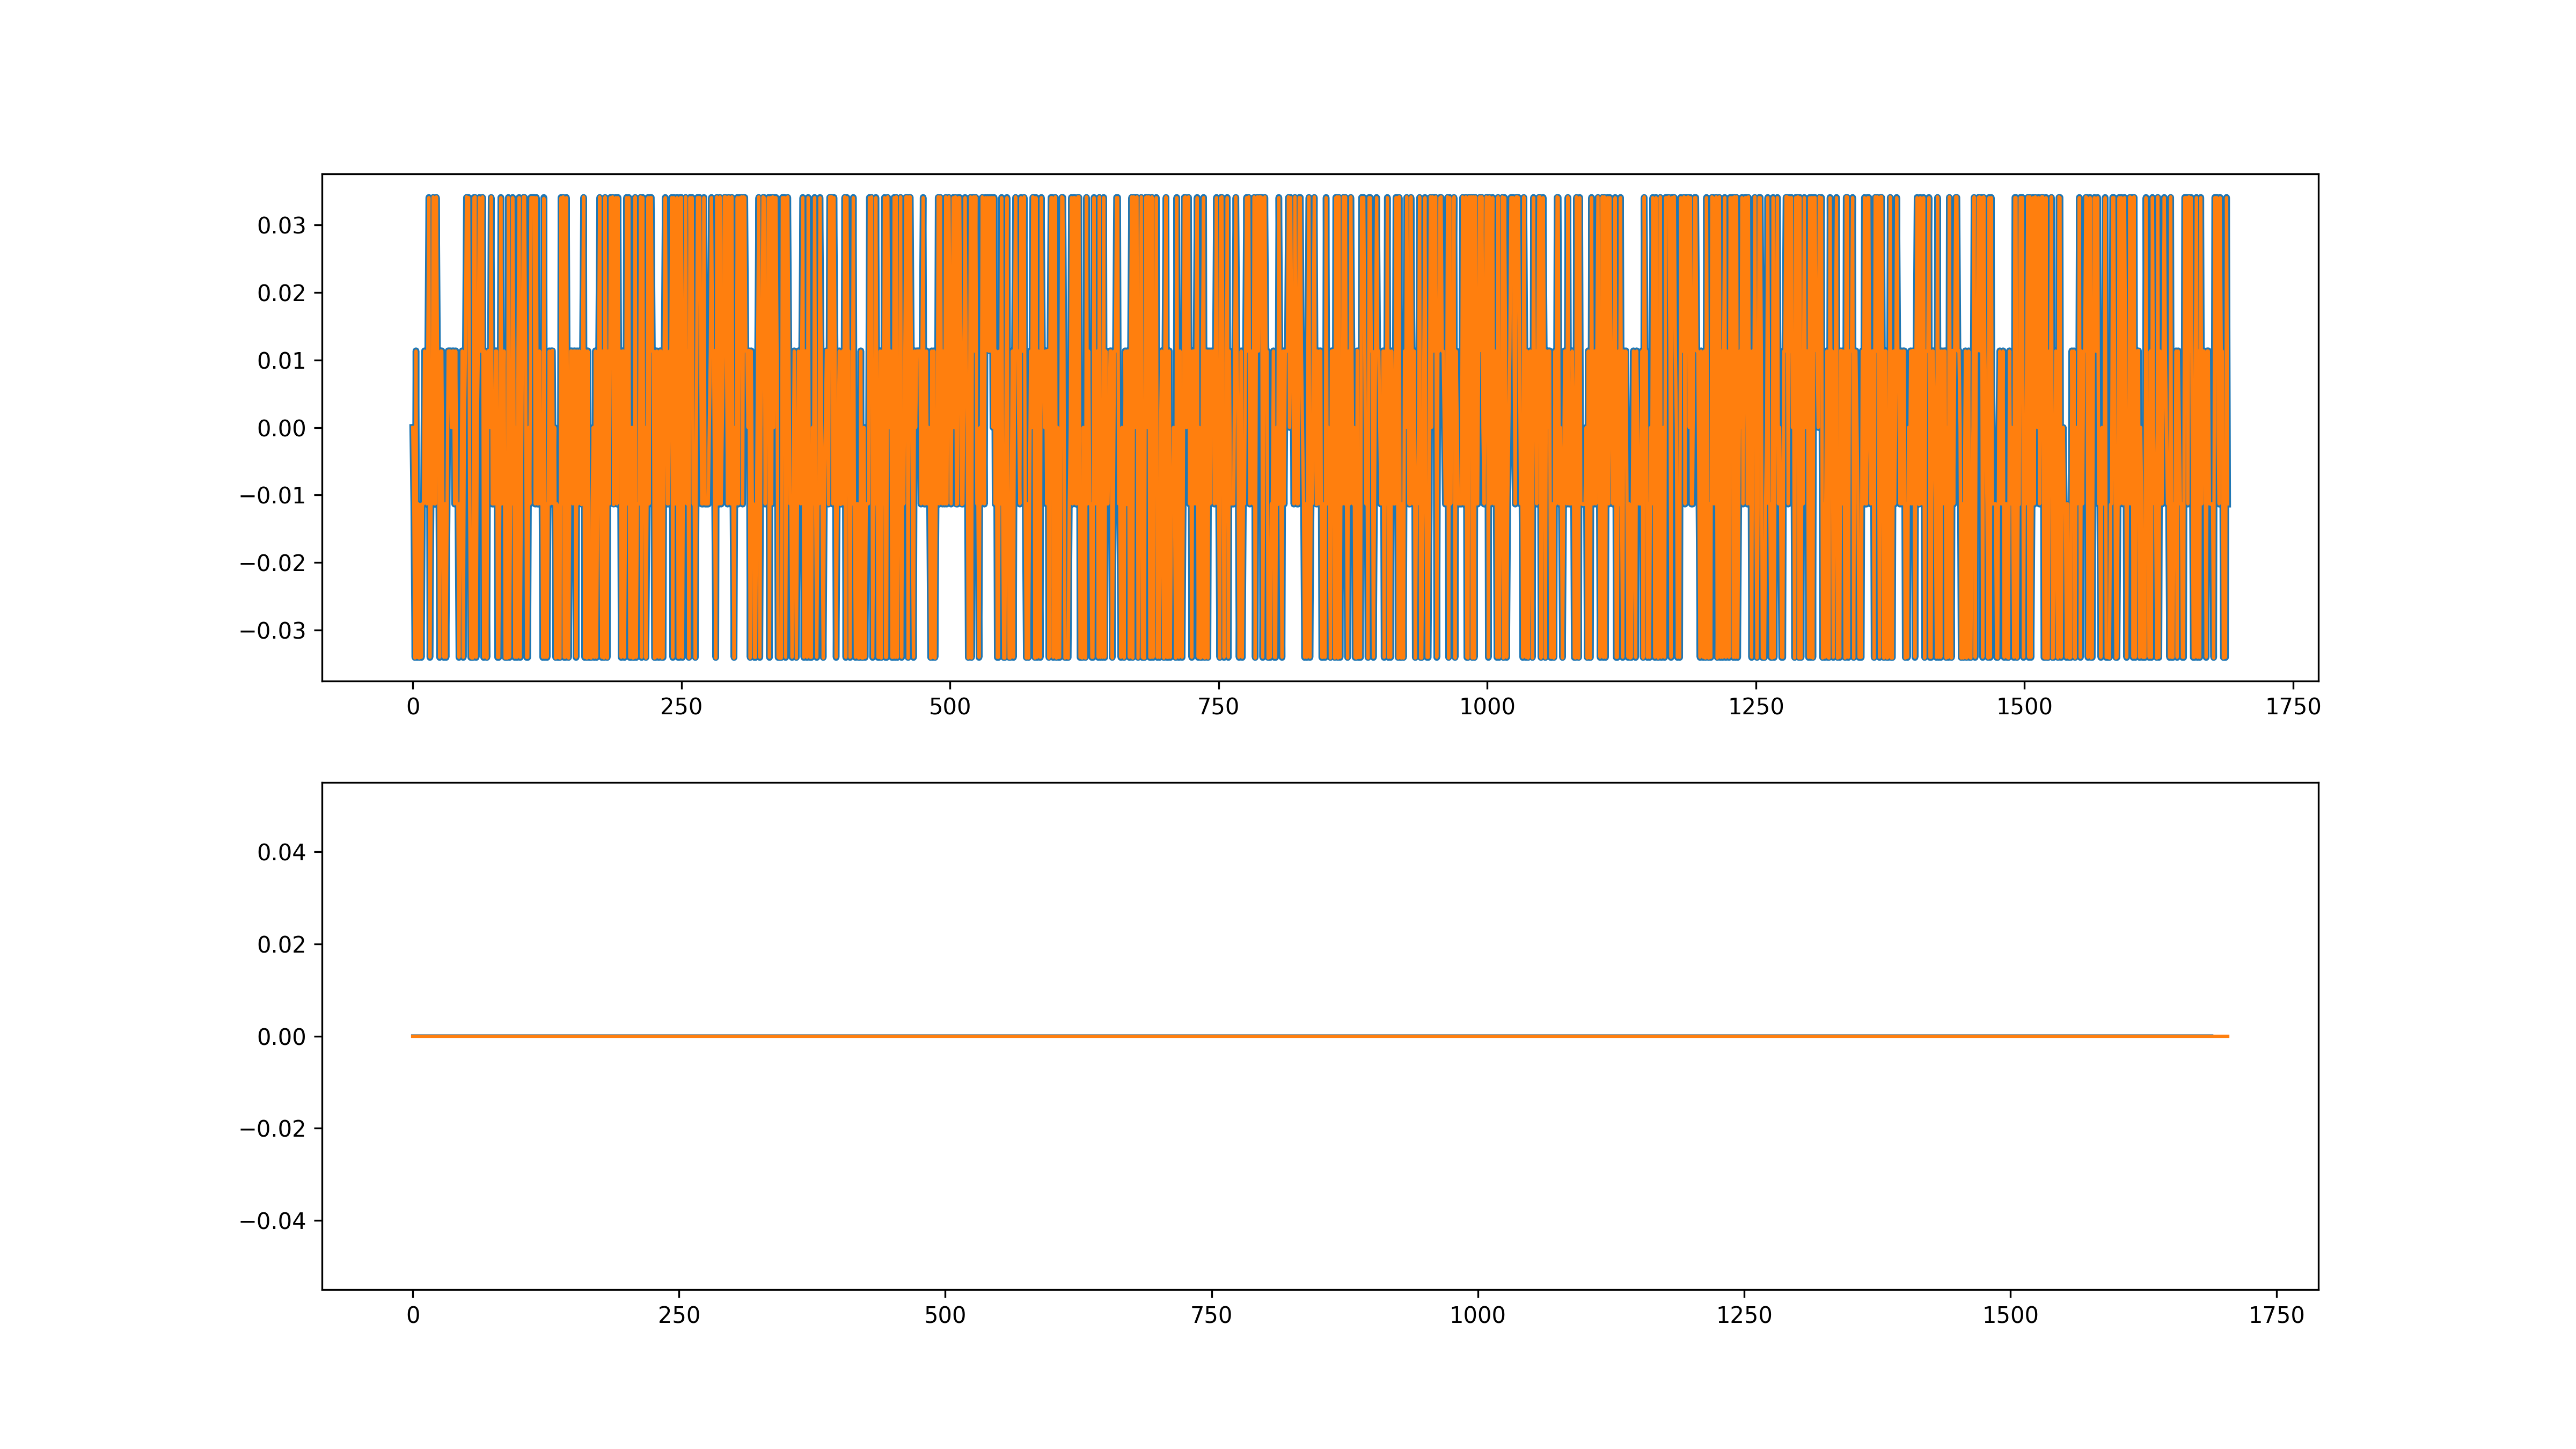
\includegraphics[width=1\columnwidth,trim={0 0.5cm 1cm 1cm},clip]{../../Linux/Trabajo/FullSystemCCTb/imgs/vsOctave2flatim.png} % Example image
	\captionof{figure}{Ecualización contra Matlab 16QAM con ruido, parte real.}
	\end{center}
	\label{eqmatlabflatim}
\end{minipage}	

Un par de cosas importantes a notar en estas dos figuras \ref{eqmatlabflatre} y \ref{eqmatlabflatim}. La primera es que el canal en la parte real arroja valores, mientras que en el imaginario es cero. Esto tiene sentido, ya que si el canal es plano su parte real valdrá una constante, y su parte imaginaria 0. A su vez, en la parte real aparecen unos picos, estos son los pilotos, que al ser equalizados vuelven a tener valores reales, por lo que no aparecen en la segunda gráfica.

Pasando ya al canal de DVBT, es muy parecido al código del canal plano, pero activando el canal. Se obtienen estos valores:

\vspace{5mm} 
\begin{minipage}{\linewidth}
	\begin{center}
	% \begin{table}[h] % [h] forces the table to be output where it is defined in the code (it suppresses floating)
	\centering % Centre the table
		\begin{tabular}{l l l l}
		\toprule
		\textit{M.F.} & \textbf{MSE [dB]} & \textbf{RMSE [dB]} & \textbf{MAE}\\
		\midrule
		BPSK 2k & $-37.6$ &  $-18.8$ & $5 \cdot 10^{-3}$ \\
		QPSK 2k& $-44.5$ &  $-22.26$ & $1.25 \cdot 10^{-3}$ \\
		16QAM 2k& $-43.8$ &  $-21.9$ & $1.4 \cdot 10^{-3}$ \\
		BPSK 8k & $-40$ &  $-20$ & $2 \cdot 10^{-3}$ \\
		QPSK 8k & $-51.8$ &  $-25.9$ & $1 \cdot 10^{-4}$ \\
		16QAM 8k& $-52.3$ &  $-26.3$ & $1\cdot 10^{-4}$ \\
		\bottomrule
	\end{tabular}
	% \caption{Sausage nutrition.}
	% \end{table}
	\captionof{table}{Resultados canal DVBT contra Matlab de las señales complejas.}
	\end{center}
	\label{tablamatlab}
\end{minipage}

donde no se ha añadido ruido.

\begin{minipage}{\linewidth}
	\begin{center}
		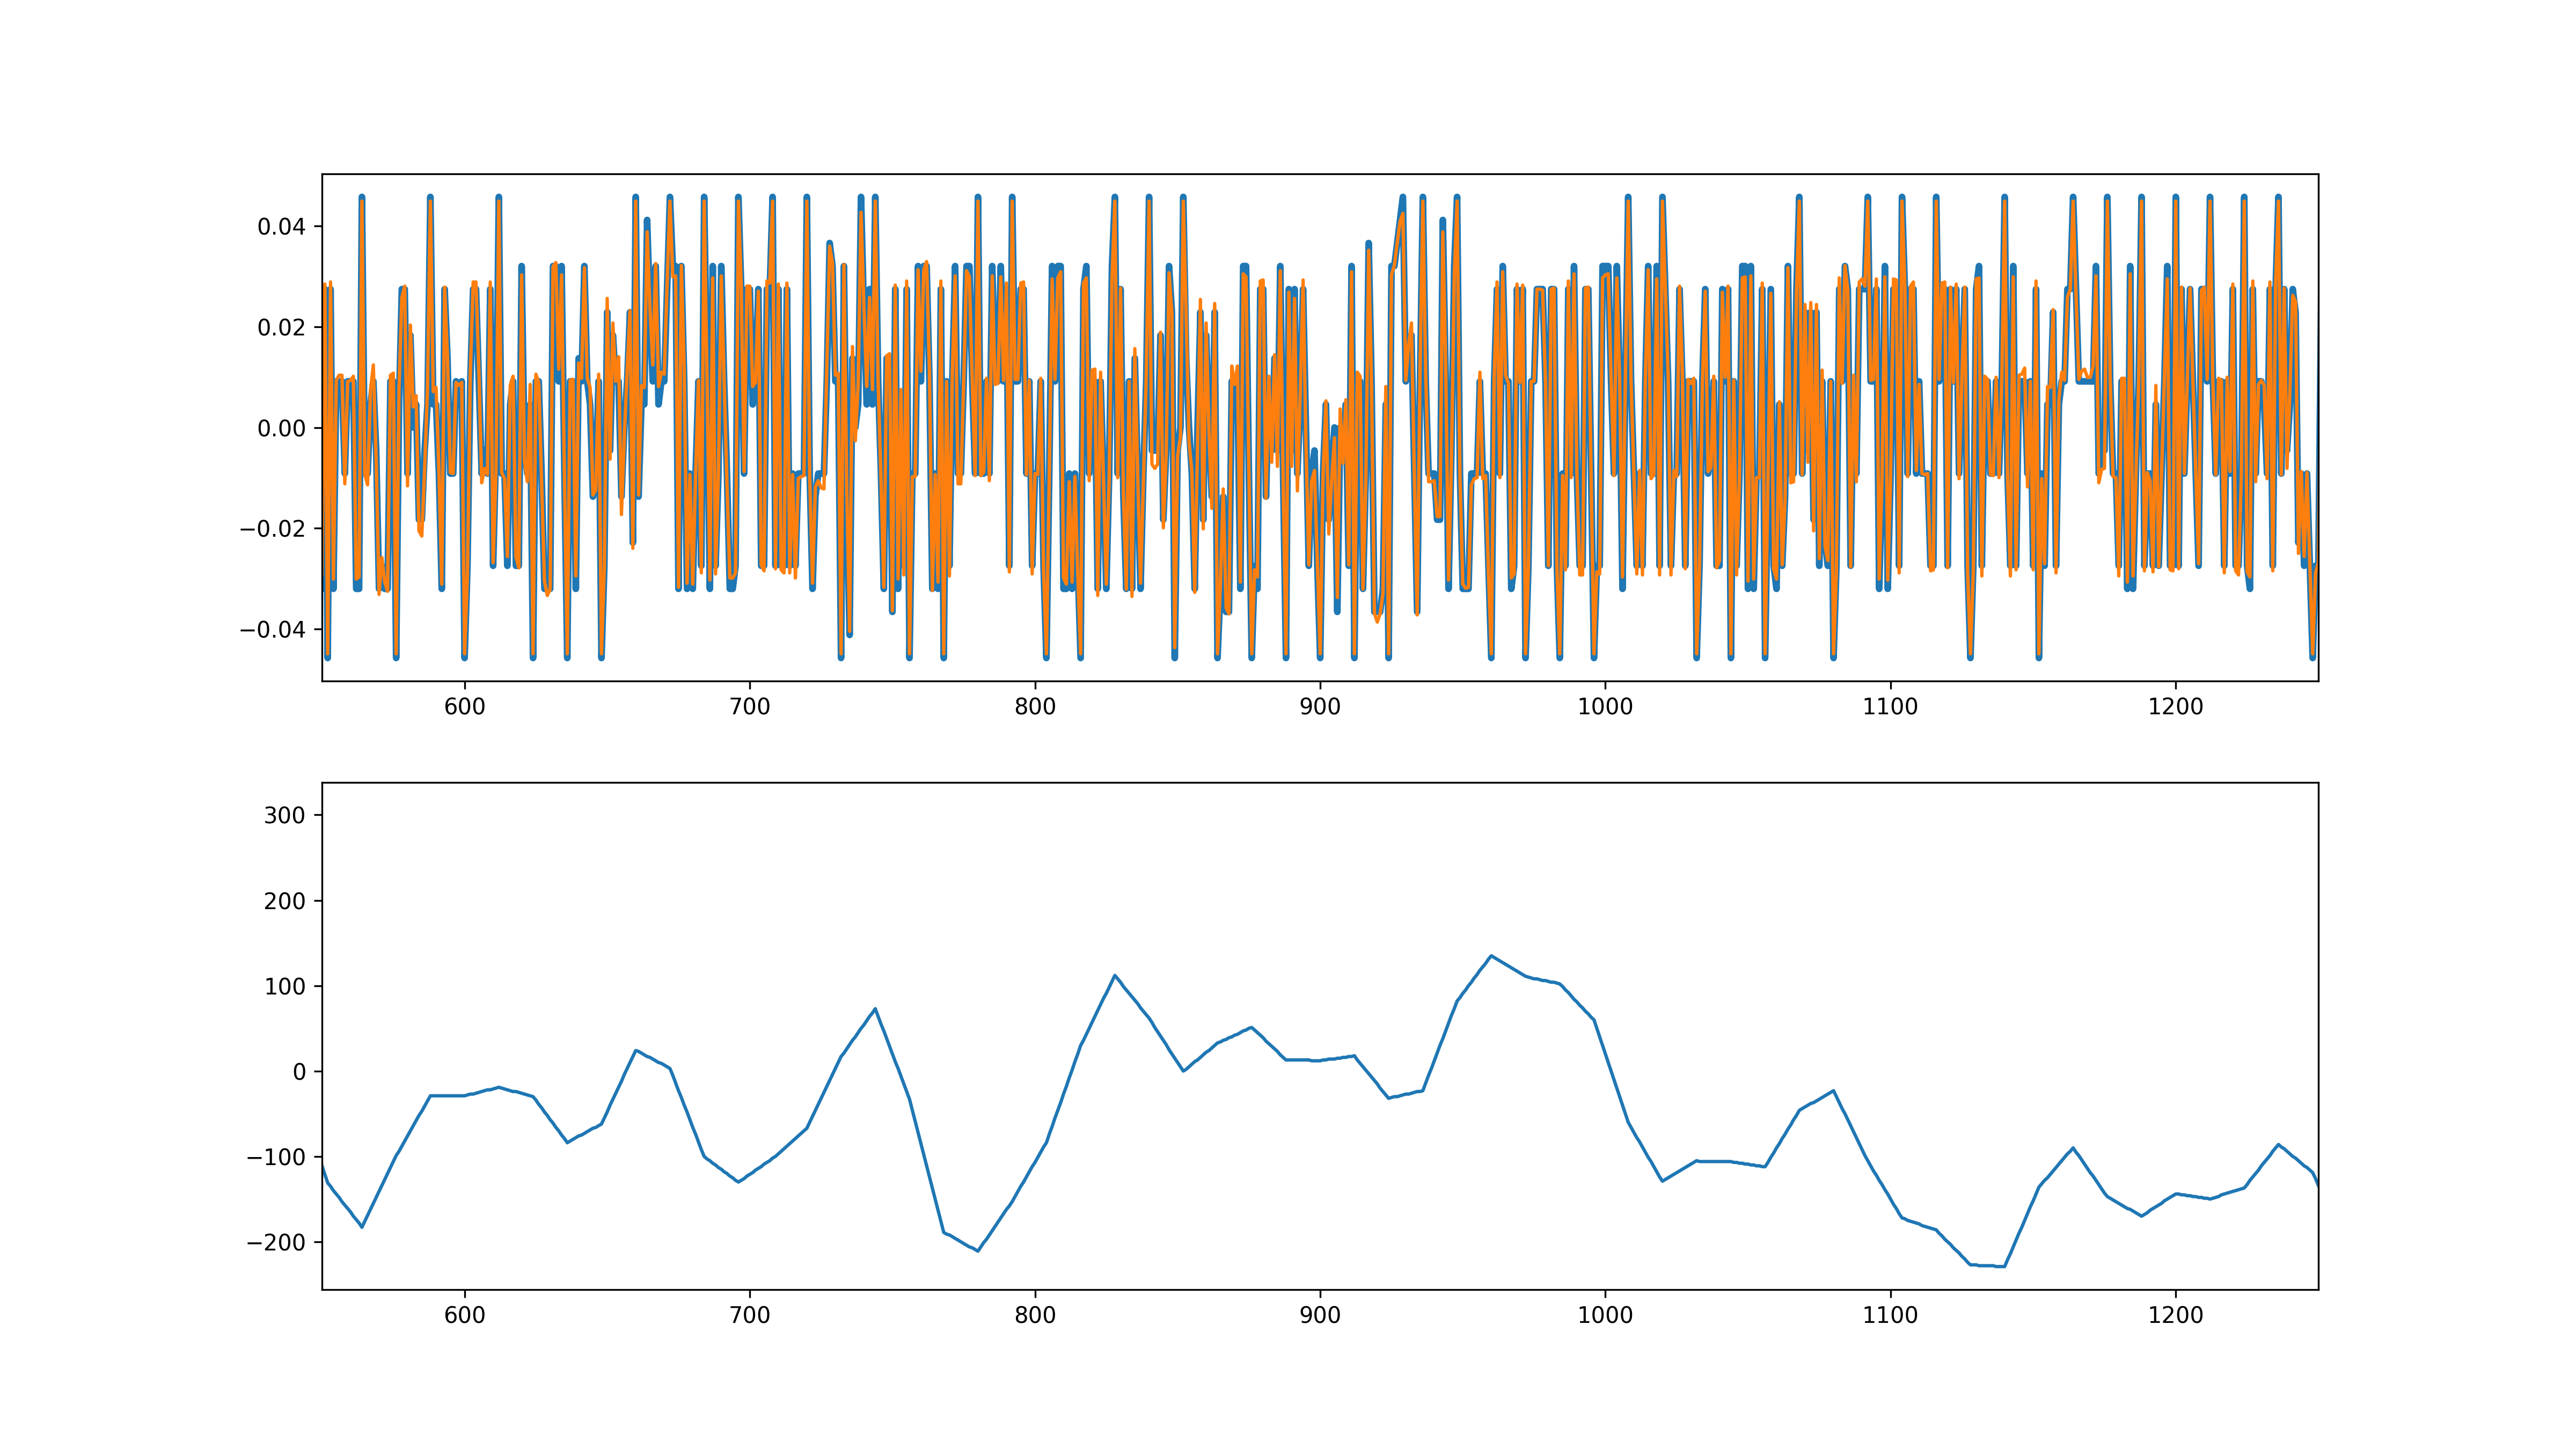
\includegraphics[width=1\columnwidth,trim={0 0.5cm 1cm 0.5cm},clip]{../../Linux/Trabajo/FullSystemCCTb/imgs/vsOctave2re.png} % Example image
	\captionof{figure}{Ecualización de la parte real modo 2k, señal de datos y estimación del canal, 16QAM.}
	\end{center}
	\label{modo2eqre}
\end{minipage}

\begin{minipage}{\linewidth}
	\begin{center}
		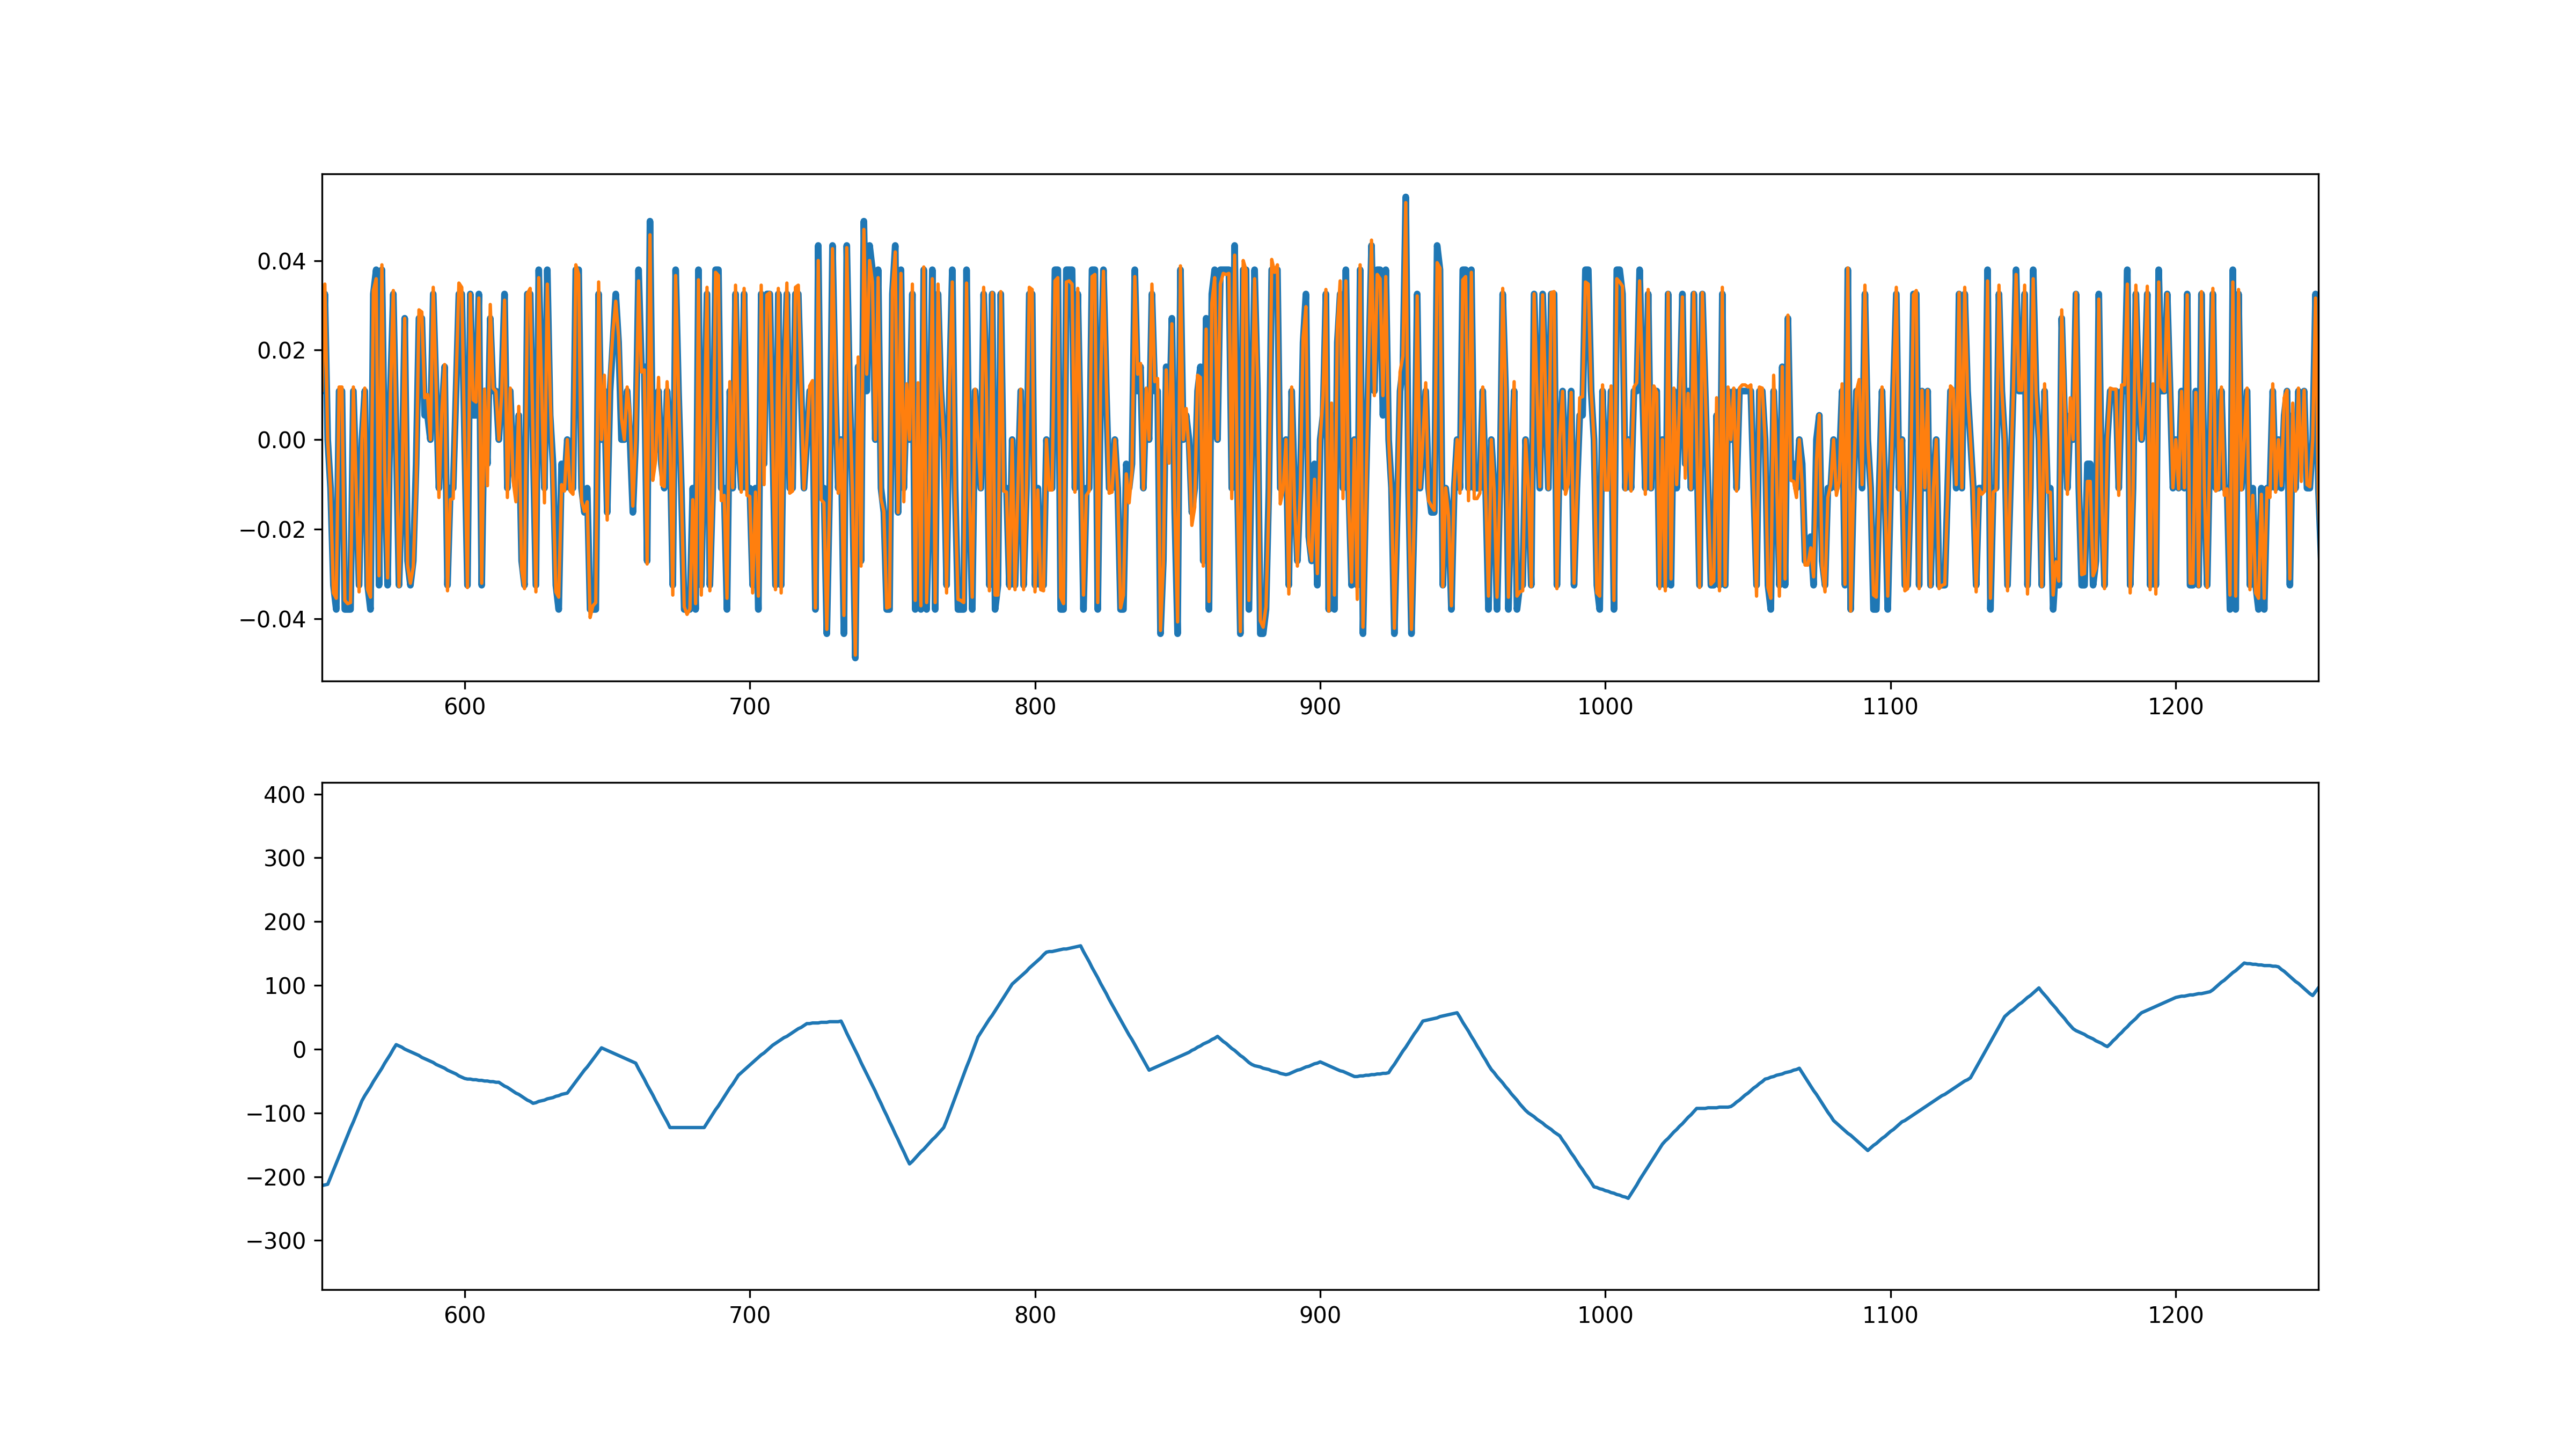
\includegraphics[width=1\columnwidth,trim={0 0.5cm 1cm 0.5cm},clip]{../../Linux/Trabajo/FullSystemCCTb/imgs/vsOctave2im.png} % Example image
	\captionof{figure}{Ecualización de la parte imaginaria modo 2k, señal de datos y estimación del canal, 16QAM.}
	\end{center}
	\label{modo2eqim}
\end{minipage}

\vspace{5mm} 
\begin{minipage}{\linewidth}
	\begin{center}
	% \begin{table}[h] % [h] forces the table to be output where it is defined in the code (it suppresses floating)
	\centering % Centre the table
		\begin{tabular}{l l l l}
		\toprule
		\textit{M.F.} & \textbf{MSE [dB]} & \textbf{RMSE [dB]} & \textbf{MAE}\\
		\midrule
		BPSK 2k & $-37.5$ &  $-18.75$ & $5 \cdot 10^{-3}$ \\
		QPSK 2k & $-44.5$ &  $-22.25$ & $1 \cdot 10^{-3}$ \\
		16QAM 2k& $-43.6$ &  $-21.8$ & $1.5 \cdot 10^{-3}$ \\
		BPSK 8k & $-40.5$ &  $-20.3$ & $1.7 \cdot 10^{-3}$ \\
		QPSK 8k & $-51.9$ &  $-25.9$ & $1 \cdot 10^{-4}$ \\
		16QAM 8k& $-48.8$ &  $-24.4$ & $2 \cdot 10^{-4}$ \\
		\bottomrule
	\end{tabular}
	% \caption{Sausage nutrition.}
	% \end{table}
	\captionof{table}{Resultados canal ruidoso DVBT contra Matlab de señales complejas.}
	\end{center}
	\label{tablamatlabruido}
\end{minipage}	

En este caso los resultados son muy similares otra vez, lo cual es lógico. La BPSK tiene peor rendimiento al estar considerando la parte imaginaria que tiene bastante más error que la real.

\subsection{Integración continua}

En el fichero de integración continua se encuentran las llamadas a todos los tests que se mueven desde la imagen docker en los runners dedicados en la universidad. Todos pertenencen al mismo \emph{stage}, \emph{test.}

Un ejemplo puede verse en la parte dedicada al sistema completo, con ecualizador.

\begin{minted}[linenos = true, frame = single]{yaml}
test_full:
  stage: test
  image: registry.gitlab.com/hgpub/fosshdl-dist:edc
  script:
    - cd Linux/Trabajo/FullSystemCCTb
    - make
  artifacts:
    when: always
    paths:
      - Linux/Trabajo/FullSystemCCTb/results.xml
      - Linux/Trabajo/FullSystemCCTb/imgs/eq.png
      - Linux/Trabajo/FullSystemCCTb/imgs/eq_rst.png
      - Linux/Trabajo/FullSystemCCTb/imgs/vsOctave2.png
      - Linux/Trabajo/FullSystemCCTb/imgs/vsOctave8.png
      - Linux/Trabajo/FullSystemCCTb/imgs/estimacioncanalyeq.png
    reports:
      junit:
        - Linux/Trabajo/FullSystemCCTb/results.xml
\end{minted}

A parte del fichero xml con los resultados de los test se extraen imágenes por si ha habido error poder ver directamente más información.

\subsection{Makefiles}

Ha sido pasado por alto pero para hacer uso de CoCoTb es necesario manejar los Makefiles, los cuales podian ser usados a través de Teros posteriormente.

Un makefile de ejemplo puede ser este, para el estimador:

\begin{minted}[linenos = true, frame = single]{bash}
#  Makefile

# defaults
SIM ?= ghdl
TOPLEVEL_LANG ?= vhdl

VHDL_SOURCES += $(PWD)/../interpolatorMig.vhd
VHDL_SOURCES += $(PWD)/../PRBS.vhd
VHDL_SOURCES += $(PWD)/../delayer.vhd
VHDL_SOURCES += $(PWD)/../contador1_12.vhd
VHDL_SOURCES += $(PWD)/../FSM.vhd
VHDL_SOURCES += $(PWD)/../toplevel.vhd

# VHDL_SOURCES_lib += $(PWD)/../edc_common.vhd

# version of GHDL
GHDL_ARGS ?= --std=08

# TOPLEVEL is the name of the toplevel module in your Verilog or VHDL file
TOPLEVEL = toplevel

SIM_ARGS +=--wave=tb_toplevel.ghw

# MODULE is the basename of the Python test file
MODULE = tb_toplevel

# include cocotb's make rules to take care of the simulator setup
include $(shell cocotb-config --makefiles)/Makefile.sim
\end{minted}

\Newpage

\section{Resumen hitos realizados}

Recogiendo todo lo mencionado anteriormente, se han realizado las siguientes tareas:

\begin{itemize}
	\item Diseño de estimador de canal OFDM desde cero con arquitectura \emph{pipeline} y retraso de solo tres ciclos de reloj.
	\item Depuración de códigos mediante la herramienta GtkWave y gráficas con pyplot.
	\item Verificación de todos los bloques usados y algunos extra que finalmente no se emplearon.
	\item Uso de CoCoTb para la mayor parte de la verificación VHDL.
	\item Aprovechamiento de la potencia de los \emph{Test Benchs} en Python para hacer uso de herramientas como \emph{Matplotlib} u \emph{Oct2Py}.
	\item Uso de Integración Continua (CI) mediante GitLab soportado por Docker con extracción de información variada.
	\item GitLab cuidado y memorias en formato README.md para leerse desde el propio GitLab.
\end{itemize}

\subsection{Tests realizados}

\begin{itemize}
	\item Test contador
	\item PRBS
	\begin{itemize}
		\item Test básico
		\item Test contra Matlab
	\end{itemize}
	\item Test FSM con alerta
	\item Test Interpolador con datos aleatorios contra Python
	\item Test Interpoladro Mig doble con reset
	\item Test AllButInterpolator
	\item TopLevel Estimador
	\begin{itemize}
		\item Test pilotos incial
		\item Test reset
		\item Test interpolación símbolos 2k
		\item Test interpolaciín símbolos 8k
	\end{itemize}
	\item Test ecualizador
	\item Test Registro
	\item Sistema completo
	\begin{itemize}
		\item Test canal plano entradas random
		\item Test reset
		\item Test matlab canal plano ruidoso 2k (varias modulaciones)
		\item Test matlab canal DVBT 2k (varias modulaciones)
		\item Test matlab canal DVBT 8k (varias modulaciones)
		\item Test matlab canal DVBT 2/8k ruidoso (varias modulaciones)
	\end{itemize}
\end{itemize}

 
% \section{Anexo: Códigos}
	
% El código VHDL será resultado en azul:

% \begin{minted}[linenos=true,bgcolor = colorVHDL, breaklines = true, frame = single]{vhdl}
	
% library IEEE;
% use IEEE.std_logic_1164.all;
% use IEEE.numeric_std.all;

% entity ejemplo is 
% port (
% 	rst : in std_logic;
% 	clk : in std_logic;
% );
% end ejemmplo;

% architecture arch_ejemplo of ejemplo is 

% 	signal ejemplo_signal : std_logic_vector(9 downto 0);

% begin

% 	sinc_process : process (clk,rst)
% 	begin

% 		if rising_edge(clk) then 
% 			null;
% 		end if;

% 	end process;

% end architecture;

% \end{minted}

% Y el de Python en negro

% % \subsection{Ejemplo Python}

% \begin{minted}[linenos=true, bgcolor = negro, breaklines = true,frame = single]{python}

% import numpy as np 
% import matplotlib.pyplot as plt 

% # definir algunas variables
% contador = 10
% maxciclos = 200
% clk = np.kron(np.ones(maxciclos),[1,0])

% def function_ejemplo(args):
% 	value = args*10

% 	return value

% for i in range(maxciclos):

% 	try:
% 		contador += 1
% 	except(e):
% 		print("Execpción ",e,"capturada")
% 	else:
% 		print(contador)

% \end{minted}

% \Newpage 

% \subsection{Contador}

% \inputmintedVHDL{../../Linux/Trabajo/Contador1_12.vhd}

% \inputmintedPy{../../Linux/Trabajo/ContadorCCTb/tb_contador1_12.py}

% \Newpage

% \subsection{Delayer}

% \inputmintedVHDL{../../Linux/Trabajo/Delayer.vhd}

% \Newpage

% \subsection{PRBS}

% \inputmintedVHDL{../../Linux/Trabajo/PRBS.vhd}

% \inputmintedPy{../../Linux/P2/CoCoTb/comparePRBSOctaveCoCoTb.py}

% \Newpage

% \subsection{FSM}

% \inputmintedVHDL{../../Linux/Trabajo/FSM.vhd}

% \inputmintedPy{../../Linux/Trabajo/FSMCCTb/tb_FSM.py}

% \Newpage

% \subsection{Interpolador}

% \inputmintedVHDL{../../Linux/Trabajo/interpolator.vhd}	

% \inputmintedPy{../../Linux/Trabajo/InterpoladorCCTb/tb_interpolator.py}

% \Newpage

% \subsection{InterMig}

% \inputmintedVHDL{../../Linux/Trabajo/interpolatorMig.vhd}

% \inputmintedPy{../../Linux/Trabajo/InterMigCCTb/tb_interMig.py}

% \Newpage

% \subsection{AllButInterpolator}

% \inputmintedVHDL{../../Linux/Trabajo/AllButInterpolator.vhd}

% \inputmintedPy{../../Linux/Trabajo/AllButInterpolatorCCTb/tb_AllButInterpolator.py}

% \Newpage

% \subsection{TopLevel (Estimador)}

% \inputmintedVHDL{../../Linux/Trabajo/TopLevel.vhd}

% \inputmintedPy{../../Linux/Trabajo/TopLevelCCTb/tb_toplevel.py}

% \newpage

% \subsection{Ecualizador}

% \inputmintedVHDL{../../Linux/Trabajo/eq.vhd}

% \inputmintedPy{../../Linux/Trabajo/EQCCTb/tb_eq.py}

% \Newpage

% \subsection{Sistema completo}

% \inputmintedVHDL{../../Linux/Trabajo/fullsystem.vhd}

% \Newpage

% % \inputmintedPy{../../Linux/Trabajo/FullSystemCCTb/tb_full.py}

% \Newpage

% \subsection{Integración continua}

% \inputminted[linenos=true, breaklines = true, frame = single]{yaml}{../../.gitlab-ci.yml}


\end{preview}




















% %----------------------------------------------------------------------------------------
% %	FIGURE EXAMPLE
% %----------------------------------------------------------------------------------------

% \section{Image Interpretation}

% \begin{figure}[h] % [h] forces the figure to be output where it is defined in the code (it suppresses floating)
% 	\centering
% 	\includegraphics[width=0.5\columnwidth]{swallow.jpg} % Example image
% 	\caption{European swallow.}
% \end{figure}

% %------------------------------------------------

% \subsection{What is the airspeed velocity of an unladen swallow?}

% While this question leaves out the crucial element of the geographic origin of the swallow, according to Jonathan Corum, an unladen European swallow maintains a cruising airspeed velocity of \textbf{11 metres per second}, or \textbf{24 miles an hour}. The velocity of the corresponding African swallows requires further research as kinematic data is severely lacking for these species.

% %----------------------------------------------------------------------------------------
% %	TEXT EXAMPLE
% %----------------------------------------------------------------------------------------

% \section{Understanding Text}

% \subsection{How much wood would a woodchuck chuck if a woodchuck could chuck wood?}

% %------------------------------------------------

% \subsubsection{Suppose ``chuck" implies throwing.}

% According to the Associated Press (1988), a New York Fish and Wildlife technician named Richard Thomas calculated the volume of dirt in a typical 25--30 foot (7.6--9.1 m) long woodchuck burrow and had determined that if the woodchuck had moved an equivalent volume of wood, it could move ``about \textbf{700 pounds (320 kg)} on a good day, with the wind at his back".

% %------------------------------------------------

% \subsubsection{Suppose ``chuck" implies vomiting.}

% A woodchuck can ingest 361.92 cm\textsuperscript{3} (22.09 cu in) of wood per day. Assuming immediate expulsion on ingestion with a 5\% retainment rate, a woodchuck could chuck \textbf{343.82 cm\textsuperscript{3}} of wood per day.

% %------------------------------------------------

% \paragraph{Bonus: suppose there is no woodchuck.}

% Fusce varius orci ac magna dapibus porttitor. In tempor leo a neque bibendum sollicitudin. Nulla pretium fermentum nisi, eget sodales magna facilisis eu. Praesent aliquet nulla ut bibendum lacinia. Donec vel mauris vulputate, commodo ligula ut, egestas orci. Suspendisse commodo odio sed hendrerit lobortis. Donec finibus eros erat, vel ornare enim mattis et.

% %----------------------------------------------------------------------------------------
% %	EQUATION EXAMPLES
% %----------------------------------------------------------------------------------------

% \section{Interpreting Equations}

% \subsection{Identify the author of Equation \ref{eq:bayes} below and briefly describe it in English.}

% \begin{align} 
% 	\label{eq:bayes}
% 	\begin{split}
% 		P(A|B) = \frac{P(B|A)P(A)}{P(B)}
% 	\end{split}					
% \end{align}

% Lorem ipsum dolor sit amet, consectetur adipiscing elit. Praesent porttitor arcu luctus, imperdiet urna iaculis, mattis eros. Pellentesque iaculis odio vel nisl ullamcorper, nec faucibus ipsum molestie. Sed dictum nisl non aliquet porttitor. Etiam vulputate arcu dignissim, finibus sem et, viverra nisl. Aenean luctus congue massa, ut laoreet metus ornare in. Nunc fermentum nisi imperdiet lectus tincidunt vestibulum at ac elit. Nulla mattis nisl eu malesuada suscipit.

% %------------------------------------------------

% \subsection{Try to make sense of some more equations.}

% \begin{align} 
% 	\begin{split}
% 		(x+y)^3 &= (x+y)^2(x+y)\\
% 		&=(x^2+2xy+y^2)(x+y)\\
% 		&=(x^3+2x^2y+xy^2) + (x^2y+2xy^2+y^3)\\
% 		&=x^3+3x^2y+3xy^2+y^3
% 	\end{split}					
% \end{align}

% Lorem ipsum dolor sit amet, consectetuer adipiscing elit. 
% \begin{align}
% 	A = 
% 	\begin{bmatrix}
% 		A_{11} & A_{21} \\
% 		A_{21} & A_{22}
% 	\end{bmatrix}
% \end{align}
% Aenean commodo ligula eget dolor. Aenean massa. Cum sociis natoque penatibus et magnis dis parturient montes, nascetur ridiculus mus. Donec quam felis, ultricies nec, pellentesque eu, pretium quis, sem.

% %----------------------------------------------------------------------------------------
% %	LIST EXAMPLES
% %----------------------------------------------------------------------------------------

% \section{Viewing Lists}

% \subsection{Bullet Point List}

% \begin{itemize}
% 	\item First item in a list 
% 		\begin{itemize}
% 		\item First item in a list 
% 			\begin{itemize}
% 			\item First item in a list 
% 			\item Second item in a list 
% 			\end{itemize}
% 		\item Second item in a list 
% 		\end{itemize}
% 	\item Second item in a list 
% \end{itemize}

% %------------------------------------------------

% \subsection{Numbered List}

% \begin{enumerate}
% 	\item First item in a list 
% 	\item Second item in a list 
% 	\item Third item in a list
% \end{enumerate}

% %----------------------------------------------------------------------------------------
% %	TABLE EXAMPLE
% %----------------------------------------------------------------------------------------

% \section{Interpreting a Table}

% \begin{table}[h] % [h] forces the table to be output where it is defined in the code (it suppresses floating)
% 	\centering % Centre the table
% 	\begin{tabular}{l l l}
% 		\toprule
% 		\textit{Per 50g} & \textbf{Pork} & \textbf{Soy} \\
% 		\midrule
% 		Energy & 760kJ & 538kJ\\
% 		Protein & 7.0g & 9.3g\\
% 		Carbohydrate & 0.0g & 4.9g\\
% 		Fat & 16.8g & 9.1g\\
% 		Sodium & 0.4g & 0.4g\\
% 		Fibre & 0.0g & 1.4g\\
% 		\bottomrule
% 	\end{tabular}
% 	\caption{Sausage nutrition.}
% \end{table}

% %------------------------------------------------

% \subsection{The table above shows the nutritional consistencies of two sausage types. Explain their relative differences given what you know about daily adult nutritional recommendations.}

% Lorem ipsum dolor sit amet, consectetur adipiscing elit. Praesent porttitor arcu luctus, imperdiet urna iaculis, mattis eros. Pellentesque iaculis odio vel nisl ullamcorper, nec faucibus ipsum molestie. Sed dictum nisl non aliquet porttitor. Etiam vulputate arcu dignissim, finibus sem et, viverra nisl. Aenean luctus congue massa, ut laoreet metus ornare in. Nunc fermentum nisi imperdiet lectus tincidunt vestibulum at ac elit. Nulla mattis nisl eu malesuada suscipit.

% %----------------------------------------------------------------------------------------
% %	CODE LISTING EXAMPLE
% %----------------------------------------------------------------------------------------

% \section{Reading a Code Listing}

% \lstinputlisting[
% 	caption=Luftballons Perl Script., % Caption above the listing
% 	label=lst:luftballons, % Label for referencing this listing
% 	language=Perl, % Use Perl functions/syntax highlighting
% 	frame=single, % Frame around the code listing
% 	showstringspaces=false, % Don't put marks in string spaces
% 	numbers=left, % Line numbers on left
% 	numberstyle=\tiny, % Line numbers styling
% 	]{luftballons.pl}

% %------------------------------------------------

% \subsection{How many luftballons will be output by the Listing \ref{lst:luftballons} above?}

% Aliquam arcu turpis, ultrices sed luctus ac, vehicula id metus. Morbi eu feugiat velit, et tempus augue. Proin ac mattis tortor. Donec tincidunt, ante rhoncus luctus semper, arcu lorem lobortis justo, nec convallis ante quam quis lectus. Aenean tincidunt sodales massa, et hendrerit tellus mattis ac. Sed non pretium nibh. Donec cursus maximus luctus. Vivamus lobortis eros et massa porta porttitor.

% %------------------------------------------------

% \subsection{Identify the regular expression in Listing \ref{lst:luftballons} and explain how it relates to the anti-war sentiments found in the rest of the script.}

% Fusce varius orci ac magna dapibus porttitor. In tempor leo a neque bibendum sollicitudin. Nulla pretium fermentum nisi, eget sodales magna facilisis eu. Praesent aliquet nulla ut bibendum lacinia. Donec vel mauris vulputate, commodo ligula ut, egestas orci. Suspendisse commodo odio sed hendrerit lobortis. Donec finibus eros erat, vel ornare enim mattis et.

% %----------------------------------------------------------------------------------------

\end{document}
